% Options for packages loaded elsewhere
\PassOptionsToPackage{unicode}{hyperref}
\PassOptionsToPackage{hyphens}{url}
\PassOptionsToPackage{dvipsnames,svgnames,x11names}{xcolor}
%
\documentclass[
  letterpaper,
  DIV=11,
  numbers=noendperiod]{scrreprt}

\usepackage{amsmath,amssymb}
\usepackage{iftex}
\ifPDFTeX
  \usepackage[T1]{fontenc}
  \usepackage[utf8]{inputenc}
  \usepackage{textcomp} % provide euro and other symbols
\else % if luatex or xetex
  \usepackage{unicode-math}
  \defaultfontfeatures{Scale=MatchLowercase}
  \defaultfontfeatures[\rmfamily]{Ligatures=TeX,Scale=1}
\fi
\usepackage{lmodern}
\ifPDFTeX\else  
    % xetex/luatex font selection
    \setmainfont[]{Times New Roman}
    \setsansfont[]{Times New Roman}
    \setmonofont[]{Courier New}
\fi
% Use upquote if available, for straight quotes in verbatim environments
\IfFileExists{upquote.sty}{\usepackage{upquote}}{}
\IfFileExists{microtype.sty}{% use microtype if available
  \usepackage[]{microtype}
  \UseMicrotypeSet[protrusion]{basicmath} % disable protrusion for tt fonts
}{}
\makeatletter
\@ifundefined{KOMAClassName}{% if non-KOMA class
  \IfFileExists{parskip.sty}{%
    \usepackage{parskip}
  }{% else
    \setlength{\parindent}{0pt}
    \setlength{\parskip}{6pt plus 2pt minus 1pt}}
}{% if KOMA class
  \KOMAoptions{parskip=half}}
\makeatother
\usepackage{xcolor}
\usepackage[top=0.5in]{geometry}
\setlength{\emergencystretch}{3em} % prevent overfull lines
\setcounter{secnumdepth}{5}
% Make \paragraph and \subparagraph free-standing
\makeatletter
\ifx\paragraph\undefined\else
  \let\oldparagraph\paragraph
  \renewcommand{\paragraph}{
    \@ifstar
      \xxxParagraphStar
      \xxxParagraphNoStar
  }
  \newcommand{\xxxParagraphStar}[1]{\oldparagraph*{#1}\mbox{}}
  \newcommand{\xxxParagraphNoStar}[1]{\oldparagraph{#1}\mbox{}}
\fi
\ifx\subparagraph\undefined\else
  \let\oldsubparagraph\subparagraph
  \renewcommand{\subparagraph}{
    \@ifstar
      \xxxSubParagraphStar
      \xxxSubParagraphNoStar
  }
  \newcommand{\xxxSubParagraphStar}[1]{\oldsubparagraph*{#1}\mbox{}}
  \newcommand{\xxxSubParagraphNoStar}[1]{\oldsubparagraph{#1}\mbox{}}
\fi
\makeatother

\usepackage{color}
\usepackage{fancyvrb}
\newcommand{\VerbBar}{|}
\newcommand{\VERB}{\Verb[commandchars=\\\{\}]}
\DefineVerbatimEnvironment{Highlighting}{Verbatim}{commandchars=\\\{\}}
% Add ',fontsize=\small' for more characters per line
\usepackage{framed}
\definecolor{shadecolor}{RGB}{241,243,245}
\newenvironment{Shaded}{\begin{snugshade}}{\end{snugshade}}
\newcommand{\AlertTok}[1]{\textcolor[rgb]{0.68,0.00,0.00}{#1}}
\newcommand{\AnnotationTok}[1]{\textcolor[rgb]{0.37,0.37,0.37}{#1}}
\newcommand{\AttributeTok}[1]{\textcolor[rgb]{0.40,0.45,0.13}{#1}}
\newcommand{\BaseNTok}[1]{\textcolor[rgb]{0.68,0.00,0.00}{#1}}
\newcommand{\BuiltInTok}[1]{\textcolor[rgb]{0.00,0.23,0.31}{#1}}
\newcommand{\CharTok}[1]{\textcolor[rgb]{0.13,0.47,0.30}{#1}}
\newcommand{\CommentTok}[1]{\textcolor[rgb]{0.37,0.37,0.37}{#1}}
\newcommand{\CommentVarTok}[1]{\textcolor[rgb]{0.37,0.37,0.37}{\textit{#1}}}
\newcommand{\ConstantTok}[1]{\textcolor[rgb]{0.56,0.35,0.01}{#1}}
\newcommand{\ControlFlowTok}[1]{\textcolor[rgb]{0.00,0.23,0.31}{\textbf{#1}}}
\newcommand{\DataTypeTok}[1]{\textcolor[rgb]{0.68,0.00,0.00}{#1}}
\newcommand{\DecValTok}[1]{\textcolor[rgb]{0.68,0.00,0.00}{#1}}
\newcommand{\DocumentationTok}[1]{\textcolor[rgb]{0.37,0.37,0.37}{\textit{#1}}}
\newcommand{\ErrorTok}[1]{\textcolor[rgb]{0.68,0.00,0.00}{#1}}
\newcommand{\ExtensionTok}[1]{\textcolor[rgb]{0.00,0.23,0.31}{#1}}
\newcommand{\FloatTok}[1]{\textcolor[rgb]{0.68,0.00,0.00}{#1}}
\newcommand{\FunctionTok}[1]{\textcolor[rgb]{0.28,0.35,0.67}{#1}}
\newcommand{\ImportTok}[1]{\textcolor[rgb]{0.00,0.46,0.62}{#1}}
\newcommand{\InformationTok}[1]{\textcolor[rgb]{0.37,0.37,0.37}{#1}}
\newcommand{\KeywordTok}[1]{\textcolor[rgb]{0.00,0.23,0.31}{\textbf{#1}}}
\newcommand{\NormalTok}[1]{\textcolor[rgb]{0.00,0.23,0.31}{#1}}
\newcommand{\OperatorTok}[1]{\textcolor[rgb]{0.37,0.37,0.37}{#1}}
\newcommand{\OtherTok}[1]{\textcolor[rgb]{0.00,0.23,0.31}{#1}}
\newcommand{\PreprocessorTok}[1]{\textcolor[rgb]{0.68,0.00,0.00}{#1}}
\newcommand{\RegionMarkerTok}[1]{\textcolor[rgb]{0.00,0.23,0.31}{#1}}
\newcommand{\SpecialCharTok}[1]{\textcolor[rgb]{0.37,0.37,0.37}{#1}}
\newcommand{\SpecialStringTok}[1]{\textcolor[rgb]{0.13,0.47,0.30}{#1}}
\newcommand{\StringTok}[1]{\textcolor[rgb]{0.13,0.47,0.30}{#1}}
\newcommand{\VariableTok}[1]{\textcolor[rgb]{0.07,0.07,0.07}{#1}}
\newcommand{\VerbatimStringTok}[1]{\textcolor[rgb]{0.13,0.47,0.30}{#1}}
\newcommand{\WarningTok}[1]{\textcolor[rgb]{0.37,0.37,0.37}{\textit{#1}}}

\providecommand{\tightlist}{%
  \setlength{\itemsep}{0pt}\setlength{\parskip}{0pt}}\usepackage{longtable,booktabs,array}
\usepackage{calc} % for calculating minipage widths
% Correct order of tables after \paragraph or \subparagraph
\usepackage{etoolbox}
\makeatletter
\patchcmd\longtable{\par}{\if@noskipsec\mbox{}\fi\par}{}{}
\makeatother
% Allow footnotes in longtable head/foot
\IfFileExists{footnotehyper.sty}{\usepackage{footnotehyper}}{\usepackage{footnote}}
\makesavenoteenv{longtable}
\usepackage{graphicx}
\makeatletter
\def\maxwidth{\ifdim\Gin@nat@width>\linewidth\linewidth\else\Gin@nat@width\fi}
\def\maxheight{\ifdim\Gin@nat@height>\textheight\textheight\else\Gin@nat@height\fi}
\makeatother
% Scale images if necessary, so that they will not overflow the page
% margins by default, and it is still possible to overwrite the defaults
% using explicit options in \includegraphics[width, height, ...]{}
\setkeys{Gin}{width=\maxwidth,height=\maxheight,keepaspectratio}
% Set default figure placement to htbp
\makeatletter
\def\fps@figure{htbp}
\makeatother
% definitions for citeproc citations
\NewDocumentCommand\citeproctext{}{}
\NewDocumentCommand\citeproc{mm}{%
  \begingroup\def\citeproctext{#2}\cite{#1}\endgroup}
\makeatletter
 % allow citations to break across lines
 \let\@cite@ofmt\@firstofone
 % avoid brackets around text for \cite:
 \def\@biblabel#1{}
 \def\@cite#1#2{{#1\if@tempswa , #2\fi}}
\makeatother
\newlength{\cslhangindent}
\setlength{\cslhangindent}{1.5em}
\newlength{\csllabelwidth}
\setlength{\csllabelwidth}{3em}
\newenvironment{CSLReferences}[2] % #1 hanging-indent, #2 entry-spacing
 {\begin{list}{}{%
  \setlength{\itemindent}{0pt}
  \setlength{\leftmargin}{0pt}
  \setlength{\parsep}{0pt}
  % turn on hanging indent if param 1 is 1
  \ifodd #1
   \setlength{\leftmargin}{\cslhangindent}
   \setlength{\itemindent}{-1\cslhangindent}
  \fi
  % set entry spacing
  \setlength{\itemsep}{#2\baselineskip}}}
 {\end{list}}
\usepackage{calc}
\newcommand{\CSLBlock}[1]{\hfill\break\parbox[t]{\linewidth}{\strut\ignorespaces#1\strut}}
\newcommand{\CSLLeftMargin}[1]{\parbox[t]{\csllabelwidth}{\strut#1\strut}}
\newcommand{\CSLRightInline}[1]{\parbox[t]{\linewidth - \csllabelwidth}{\strut#1\strut}}
\newcommand{\CSLIndent}[1]{\hspace{\cslhangindent}#1}

\usepackage{booktabs}
\usepackage{longtable}
\usepackage{array}
\usepackage{multirow}
\usepackage{wrapfig}
\usepackage{float}
\usepackage{colortbl}
\usepackage{pdflscape}
\usepackage{tabu}
\usepackage{threeparttable}
\usepackage{threeparttablex}
\usepackage[normalem]{ulem}
\usepackage{makecell}
\usepackage{xcolor}
\usepackage{caption}
\usepackage{anyfontsize}
\usepackage{amsmath}
\usepackage{float}
\usepackage{pdflscape}
\usepackage{afterpage}
\usepackage{longtable}
\usepackage[table]{xcolor}
\usepackage{longtable}
\usepackage{booktabs}
\usepackage{graphicx}
\usepackage{fontspec}
\setmainfont{Times New Roman}
\setsansfont{Times New Roman}
\setmonofont{Courier New}
\KOMAoption{captions}{tableheading}
\makeatletter
\@ifpackageloaded{bookmark}{}{\usepackage{bookmark}}
\makeatother
\makeatletter
\@ifpackageloaded{caption}{}{\usepackage{caption}}
\AtBeginDocument{%
\ifdefined\contentsname
  \renewcommand*\contentsname{Table of contents}
\else
  \newcommand\contentsname{Table of contents}
\fi
\ifdefined\listfigurename
  \renewcommand*\listfigurename{List of Figures}
\else
  \newcommand\listfigurename{List of Figures}
\fi
\ifdefined\listtablename
  \renewcommand*\listtablename{List of Tables}
\else
  \newcommand\listtablename{List of Tables}
\fi
\ifdefined\figurename
  \renewcommand*\figurename{Figure}
\else
  \newcommand\figurename{Figure}
\fi
\ifdefined\tablename
  \renewcommand*\tablename{Table}
\else
  \newcommand\tablename{Table}
\fi
}
\@ifpackageloaded{float}{}{\usepackage{float}}
\floatstyle{ruled}
\@ifundefined{c@chapter}{\newfloat{codelisting}{h}{lop}}{\newfloat{codelisting}{h}{lop}[chapter]}
\floatname{codelisting}{Listing}
\newcommand*\listoflistings{\listof{codelisting}{List of Listings}}
\makeatother
\makeatletter
\makeatother
\makeatletter
\@ifpackageloaded{caption}{}{\usepackage{caption}}
\@ifpackageloaded{subcaption}{}{\usepackage{subcaption}}
\makeatother

\ifLuaTeX
  \usepackage{selnolig}  % disable illegal ligatures
\fi
\usepackage{bookmark}

\IfFileExists{xurl.sty}{\usepackage{xurl}}{} % add URL line breaks if available
\urlstyle{same} % disable monospaced font for URLs
\hypersetup{
  colorlinks=true,
  linkcolor={blue},
  filecolor={Maroon},
  citecolor={Blue},
  urlcolor={Blue},
  pdfcreator={LaTeX via pandoc}}


\author{}
\date{}

\begin{document}

\begin{titlepage}
\begin{center}
\vspace*{1cm}

{\Huge \textbf{Kvantitativ metode og statistikk (IDR4000)}}

\vspace{1cm}
{\Large Kandidatnummer: 505}

\vspace{1cm}
Antall ord: \textbf{12874} % Setter inn ordtellingen her

\vspace{5cm}

\includegraphics[width=1.6\textwidth]{logo.png}

\vfill
{\large 2024-11-22}

\end{center}
\end{titlepage}

\renewcommand*\contentsname{Table of contents}
{
\hypersetup{linkcolor=}
\setcounter{tocdepth}{2}
\tableofcontents
}

\bookmarksetup{startatroot}

\chapter*{Forord}\label{forord}
\addcontentsline{toc}{chapter}{Forord}

\markboth{Forord}{Forord}

Denne rapporten inneholder ulike arbeidskrav som er gjennomført gjennom
høsten 2024.

Arbeidskravene er satt sammen og danner nå mappeeksamen i Kvantitativ
metode og statistikk (IDR4000).

Takk til Ole for mye godt samarbeid underveis, både med kode og som
selskap under ferdigstillingen av eksamen.

Lenke som gjør det mulig å etterprøve koder:
https://github.com/Eskilstrand/Mappeeksamen.git

\bookmarksetup{startatroot}

\chapter{Reliabilitetstesting}\label{reliabilitetstesting}

\section{Introduksjon}\label{introduksjon}

Reliabilitet er en utrolig viktig faktor innenfor fysiologisk testing.
Hvis man ønsker å følge utviklingen til en utøver over en lenger periode
er det viktig at testen vi benytter oss av, og utstyret som brukes i
testen måler tilnærmet likt hver gang. Hvis testene som blir brukt har
høy reliabilitet kan utøvere og trenere stole på at forskjellene i
resultater mellom ulike tester skyldes endringer i fysiologiske faktorer
og at det ikke er feilmålinger som gir utslag.

For å i ettertid kunne evaluere effekten av en treningsplan,
intervensjon eller periode må man kunne stole på testene som blir
gjennomført. Dersom testene som blir benyttet har lav reliabilitet, kan
det være vanskelig å skille mellom virkelige prestasjonsforbedringer og
tilfeldige variasjoner som skyldes unøyaktighet i målingene. Dette kan
resultere i at man endrer et godt fungerende treningsopplegg, eller at
man fortsetter med et dårlig fungerende treningsopplegg.

I idrettsvitenskapen forskes det gjerne på effekt av ulike
intervensjoner. Uavhengig av om det gjøres forskning på utrente eller
elite-utøvere er det viktig at målingene har høy reliabilitet. Dette med
bakgrunn i at vi vil levere god kvalitet i forskningen og at det skal
være litteratur man skal kunne stole på.

Det ble gjennomført fire testdager 28.08.2024, 29.08.2024, 9.09.2024 og
11.09.2024 for å teste \(\dot{V}O_{2maks}\). Formålet med disse testene
var å øve på å kunne gjennomføre fysiologiske tester med høy
reliabilitet. Reliabilitet refererer til graden av konsistens eller
pålitelighet i målinger evnen til å kunne
reprodusere\textsuperscript{1}, et eksempel på dette er ved fysiologisk
testing som repeteres i forskningsprosjekter, der bedre reliabilitet vil
indikere hvor god presisjonen er og måling av endring over
tid\textsuperscript{1}. Det er mange begreper som er relevante for å
kunne si noe om reliabilitet, men standardavviket er et av disse.
Standardavviket sier noe om hvor langt unna verdiens gjennomsnittlige
avstand er fra gjennomsnittet\textsuperscript{2}.

Kroppens maksimale oksygenopptak (\(\dot{V}O_{2maks}\)) sier noe om
kroppens maksimale evne til å ta opp og omsette
oksygen\textsuperscript{3}. \(\dot{V}O_{2maks}\) kan beskrives ved hjelp
av Ficks likning: \(\dot{V}O_{2maks}\)=MVmaks x a-vO2differansemaks.
\(\dot{V}O_{2maks}\) måles ved at man måler hvor mye oksygen kroppen
klarer å omsette pr minutt\textsuperscript{3}. Det finnes ulike måter og
fremstille \(\dot{V}O_{2maks}\) på, de to av disse er absolutt
\(\dot{V}O_{2maks}\) beskrevet som (ml ×min-1) eller relative tall
relatert til kroppsvekt (ml/kg/min).

I resultatdelen har vi valgt å bruke relativ \(\dot{V}O_{2maks}\) for å
beregne reliabiliteten til testene vi har gjennomført. Vi har også valgt
å se på sammenhengen mellom relativ \(\dot{V}O_{2maks}\) og wattmaks
under \(\dot{V}O_{2maks}\)-testen. Forskning viser at høy
\(\dot{V}O_{2maks}\), sammen med god mekanisk effektivitet og høy
laktatterskel gir bedre utholdenhetsprestasjoner, noe som reflekteres i
høyere Wmaks/kg\textsuperscript{4}.

\section{Metode}\label{metode}

\(\dot{V}O_{2maks}\)-testen ble gjennomført på en ergometersykkel med
bukkestyre (Lode Excalibur Sport; Lode B.V., Groningen, Nederland).
Kranken kalibreres på Lode-sykkelen før hver teststart. Dette gjøres for
å få nøyaktige tråkkdata på hver forsøksperson. Sykkel stilles inn etter
utøvers ønske for å sikre best mulig sittestilling ved første test.
Sykkel stilles inn etter nøyaktig samme mål ved senere tester for å
gjøre reliabiliteten høy. For å måle det maksimale oksygenopptaket ble
det brukt Vyntus (Jaeger Vyntus CPX, Hoechberg, Tyskland).
Gassanalysator kalibreres til \textless{} 2,0\% differanse og luftvolum
kalibreres til \textless{} 0,2\% differanse. Syklistene veies med de
klærne de skal sykle med, og 0,3kg trekkes fra (300g er et estimat på
vekten av klærne forsøkspersonen har på). For å kunne sikre god
relabilitet ble det tydeliggjort at man skulle replisere det siste
måltidet før test, ha det samme koffeininntaket, avstå fra alkohol og
tobakk de siste 72 timene før test og prøve å få tilnærmet lik søvn,
samt trene det samme dagen før test. Da dette er faktorer som kan spille
inn på prestasjon og metabolismen\textsuperscript{5} og dermed påvirke
relabiliteten.

\(\dot{V}O_{2maks}\)-testen gjennomføres etter en fem minutters
standardisert oppvarming på ergometersykkelen. Oppvarmingen starter to
minutter på 11-12 i Borg, deretter to minutter på 15 i Borg før ett
minutt på 11-12 Borg. Testen starter på en belastning (Watt) basert på
deltagerens nivå i samråd med utøver og testleder. Det viktigste er at
påfølgende \(\dot{V}O_{2maks}\) tester starter på samme watt.
Wattbelastningen økte med 20W eller 25W (20W for kvinne og 25W for mann)
hvert minutt frem til utøveren når maksimal utmattelse. Maksimal
utmattelse ble i denne sammenheng ikke evne til å kunne opprettholde RPM
\textgreater{} 60. Under \(\dot{V}O_{2maks}\) var RPM valgfritt.
Testleder gjør verbal oppmuntring og sekundering underveis i testen. For
at verbal oppmuntring og instruksjon ved test skulle være lik etterstreb
vi å ha samme testleder til samme forsøksperson\textsuperscript{6}. Det
blir registrert nye oksygenmålinger hvert 30 sek, og de to høyeste
påfølgende målingene blir definert som \(\dot{V}O_{2maks}\). Umiddelbart
etter test oppgir utøveren opplevd anstrengelse på Borg skala. Maks
hjertefrekvens blir lest av fra utøvers pulsklokke. Blodprøve ble tatt
fra utøverens fingertupp 1 min etter endt test for å måle {[}BLa-{]}.
{[}BLa-{]} blir deretter målt ved hjelp av en Biosen C-line (Biosen
C-line Lactate Analyzer, EKF Diagnostic GmbH, Barleben, Germany). Etter
endt test ble det hentet ut data som videre ble plottet inn i Excel og
videre ført statistikk på ved hjelp av Rstudio.

\section{Resultat}\label{resultat}

Etter at testene er gjennomført kan vi se nærmere på hver forsøkperson
sine data, ved T1. T1 er valgt da denne testen hadde flest deltakere.
Dette gir muligheten til å se på hver enkelt forsøksperson om man finner
dette interessant (Table~\ref{tbl-tbl1}). Verdiene man kan se i
tabellen, er verdier som er plottet etter endt
\(\dot{V}O_{2maks}\)-test.

\begin{table}

\caption{\label{tbl-tbl1}}

\centering{

[H]
\centering\begingroup\fontsize{6}{8}\selectfont

\begin{tabular}{l>{\raggedright\arraybackslash}p{0.5cm}>{\raggedright\arraybackslash}p{0.5cm}>{\raggedright\arraybackslash}p{0.5cm}>{\raggedright\arraybackslash}p{0.5cm}>{\raggedright\arraybackslash}p{0.5cm}>{\raggedright\arraybackslash}p{0.5cm}>{\raggedright\arraybackslash}p{0.5cm}>{\raggedright\arraybackslash}p{0.5cm}>{\raggedright\arraybackslash}p{0.5cm}>{\raggedright\arraybackslash}p{0.5cm}>{\raggedright\arraybackslash}p{0.5cm}>{\raggedright\arraybackslash}p{0.5cm}>{\raggedright\arraybackslash}p{0.5cm}>{\raggedright\arraybackslash}p{0.5cm}>{\raggedright\arraybackslash}p{0.5cm}>{\raggedright\arraybackslash}p{0.5cm}}
\toprule
\textbf{Parameter} & \textbf{1} & \textbf{2} & \textbf{3} & \textbf{4} & \textbf{5} & \textbf{6} & \textbf{7} & \textbf{8} & \textbf{9} & \textbf{10} & \textbf{11} & \textbf{12} & \textbf{13} & \textbf{14} & \textbf{15} & \textbf{16}\\
\midrule
Borg$_{max}$ & 19.2 (0.96) & 19 (0.82) & 18 (1.2) & 19 (0) & 19.5 (0.71) & 19 (0) & 17.5 (1.7) & 17 (NA) & 19.7 (0.58) & 20 (0) & 17.5 (0.71) & 18 (1.7) & 18.3 (0.58) & 18.8 (0.5) & 17 (1) & 19.5 (0.71)\\
VO$_{2max}$ (ml/kg/min) & 33.5 (1.5) & 43.7 (2.6) & 51.6 (4.1) & 37.1 (1.1) & 58.9 (0.64) & 45.5 (0.2) & 61.8 (1.9) & 43.5 (NA) & 58.8 (0.59) & 43.2 (0.89) & 56.5 (0.94) & 61.7 (3.1) & 51.3 (0.88) & 65.7 (1.1) & 39.8 (2.6) & 60.2 (1.2)\\
Watt/kg & 2.5 (0.14) & 3.58 (0.044) & 3.6 (0.46) & 3 (0.2) & 5.18 (0.082) & 3.51 (0.1) & 5.24 (0.2) & 3.93 (NA) & 4.92 (0.038) & 3.76 (0.014) & 4.93 (0.049) & 5.6 (0.4) & 3.87 (0.062) & 5.51 (0.1) & 2.85 (0.12) & 4.63 (0.065)\\
VO$_{2max}$ (ml/min) & 3240 (150) & 2700 (160) & 4130 (300) & 2860 (52) & 4390 (48) & 3710 (6.4) & 5130 (140) & 2540 (NA) & 4650 (41) & 3100 (64) & 3640 (97) & 4480 (230) & 4590 (48) & 4520 (59) & 4100 (270) & 4960 (130)\\
Watt$_{max}$ & 243 (13) & 221 (2.8) & 288 (36) & 231 (13) & 387 (6.1) & 286 (7.5) & 435 (19) & 230 (NA) & 389 (2.1) & 269 (1.2) & 318 (0) & 407 (29) & 347 (6.9) & 380 (5.7) & 293 (12) & 382 (3.1)\\
\bottomrule
\multicolumn{17}{l}{\textsuperscript{} Table 1.1: Tabellen viser hver deltakers gjennomsnitt og standardavvik i () på verdier vi har undersøkt}\\
\end{tabular}
\endgroup{}

}

\end{table}%

Etter å ha gjennomført VO\textsubscript{2maks}-testene ser vi at
kvinnene på 1MAIDR har et gjennomsnittlig oksygenopptak på 3163 ± 484.
Mennene har derimot et gjennomsnittlig oksygenopptak på 4380 ± 515.

Reliabiliteten mellom t1 og t2 er 2.47\%, mens reliabiliteten mellom t3
og t4 er 4.78\%.

\subsection{\texorpdfstring{Korrelasjon mellom
\textbf{\(\dot{V}O_{2maks}\)} og Wattmaks per
kg}{Korrelasjon mellom \textbackslash dot\{V\}O\_\{2maks\} og Wattmaks per kg}}\label{korrelasjon-mellom-dotvo_2maks-og-wattmaks-per-kg}

\begin{figure}[H]

{\centering 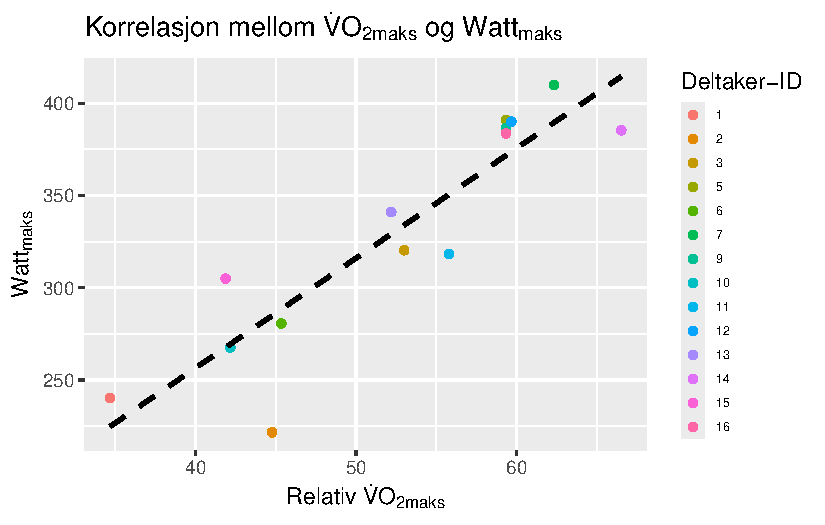
\includegraphics{01-reliability-tools_files/figure-pdf/unnamed-chunk-10-1.pdf}

}

\caption{Hvert punkt = én observasjon}

\end{figure}%

\section{Diskusjon}\label{diskusjon}

På bakgrunn av resultatene vi har observert under testing av
\(\dot{V}O_{2maks}\), kan man slå fast at reliabiliteten til metoden vi
har brukt er ganske god. Resultatene tyder på at vi får målt det vi er
ute etter på en god måte, og det vil variere lite i måle-utstyret fra
gang til gang.

Dette sikrer at vi med ganske god sikkerhet, kan fastslå om et
treningsprogram fungerer, ved å gjøre repeterte tester, med
treningsperioder i mellom.

\bookmarksetup{startatroot}

\chapter{Regresjonsmodeller og
prediksjoner}\label{regresjonsmodeller-og-prediksjoner}

\section{Introduksjon}\label{introduksjon-1}

En regresjonsmodell er en modell som kvantifiserer forholdet mellom en
eller flere uavhengige variabler og en avhengig variabel. Innen medisin
er regresjon den analysemtoden som er hyppigst anvendt. Det finnes
forskjellige regresjonsmodeller. De vanligste er lineær regresjon,
polynominal regresjon og logistisk regresjon. Hva man har av datasett
vil bestemme hvilken regresjonsmodell som egner seg best å
benytte\textsuperscript{7}.

En lineær regresjonsmodell er en modell der en kan estimere verdien av
en avhengig variabel basert på verdien av andre kjente uavhengige
variabler\textsuperscript{7}. I en slik modell benyttes en rett linje
for å lage en modell som beskriver dataen. Følgende funksjon benyttes
for å skape det lineære plottet:

y\textsubscript{i} = b\textsubscript{0} +
b\textsubscript{1}x\textsubscript{i} + e\textsubscript{i}

der y\textsubscript{i} er den avhengige variabelen som kan estimeres ved
å benytte de uavhengige variablene b\textsubscript{1}x\textsubscript{i}
og b\textsubscript{0}. b\textsubscript{0} er skjæringspunktet til grafen
og b\textsubscript{1} er stigningstallet til grafen.

Laktatterskeltesting er en sentral metode innen prestasjonsanalyse og
treningsoptimalisering, spesielt i utholdenhetsidretter. Laktatterskelen
representerer den høyeste intensiteten hvor kroppen kan opprettholde
balanse mellom produksjon og eliminering av laktat i blodet. Dette er en
viktig parameter for å forstå hvordan kroppen responderer på økende
treningsintensitet, og den gir verdifull innsikt i både fysisk kapasitet
og treningsprogrammering.

For å bestemme laktatterskelen benyttes typisk en trinnvis økning i
treningsintensitet mens blodprøver tas for å måle laktatnivåer.
Relasjonen mellom treningsintensitet og blodlaktat analyseres deretter
ved hjelp av regresjonsmodeller for å estimere intensitetsnivåene ved
faste laktatkonsentrasjoner, ofte 2 og 4 mmol/L. Disse tersklene gir
grunnlag for å skille mellom moderat og høy intensitet i trening, noe
som er avgjørende for å optimalisere treningsplaner\textsuperscript{8}.

\section{Part 1 - Lactate thresholds}\label{part-1---lactate-thresholds}

\subsection{Metode}\label{metode-1}

Dataene ble organisert i et mer hensiktsmessig format (tidy data) for å
forenkle videre analyse og modellering. Deretter ble ulike
regresjonsmodeller anvendt for å representere dataene. Nye
skjæringspunkter ble tegnet opp for å illustrere treningsintensitet ved
forskjellige laktatnivåer.

\subsection{Resultat}\label{resultat-1}

\begin{figure}[H]

\centering{

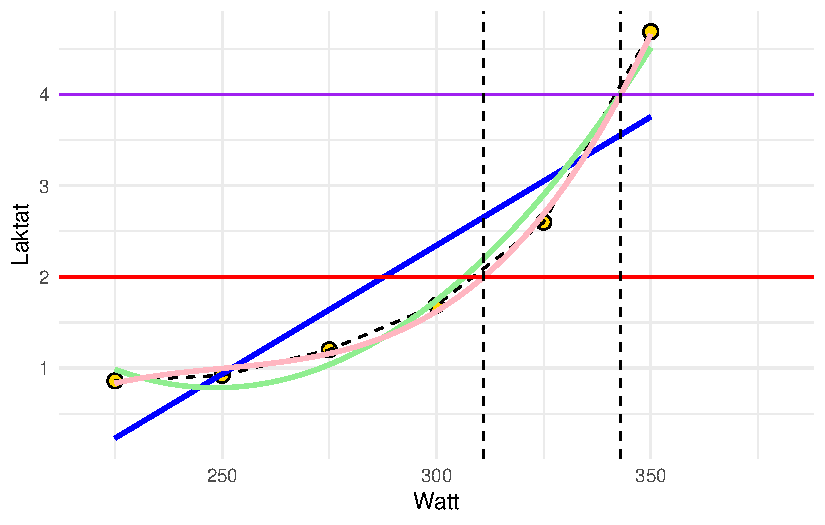
\includegraphics{02-regression-models_files/figure-pdf/fig-fig1-1.pdf}

}

\caption{\label{fig-fig1}Figur 1: Gule punkter: laktat og watt, blå
linje: lineær regresjon, lysegrønn: andregradsligning, rosa:
tredjegradsligning.}

\end{figure}%

Vår beste prediksjon til belastningen på 2 mmol \textbf{×} L-1 er 311W,
denne kommer fra tredjegradsligningen. Den predikerte belastningen fra
en lineær modell gir 288W. For predikert terskelwatt (4 mmol \textbf{×}
L-1) gir tredjegradsligningen 343W, som er den beste prediksjonen, mens
den lineære modellen gir et estimat på 359W.

\subsection{Diskusjon}\label{diskusjon-1}

Vi har valgt å se på subject 10 fra datasettet Cyclingstudy. Vi gjør om
datasettet til tidydata. Dette gjør vi for å gi watt og laktat hver sine
verdier. Vi plotter inn laktatverdier og wattverdier (gule punkter).
Deretter tegner vi en stiplet linje som følger punktene. Vi gjør en
regresjonsanalyse, først en lineær modell (blå linje), deretter en
andregradsligning (grønn) og til slutt en tredjegradsligning (rosa).
Disse bruker vi for å observere hvilken modell som passer best i dette
tilfellet.

For å understreke hvor unøyaktig den lineære modellen er i dette
tilfellet, kan man på øyemål se at laktaten på 300W viser omtrent 2.4
mmol \textbf{×} L-1. Den faktiske laktaten på 300W er 1.69 mmol
\textbf{×} L-1 (Figure~\ref{fig-fig1}).

\section{Part 2 - Predicting sizes of DNA
fragments}\label{part-2---predicting-sizes-of-dna-fragments}

\subsection{Metode}\label{metode-2}

For å predikere kalibreringskurven til qPCR, må en rekke prosesser på
molekylærlaboratoriet gjennomføres før dataene kan analyseres i R
Studio.

For å utføre en PCR på en 2\% agarosegel, ble det først tatt helblod fra
en forsøksperson for å ekstrahere DNA. Helblodet gjennomgikk ulike
prosesser hvor forskjellige løsninger og primere ble tilsatt. Dette
resulterte i et PCR-produkt. En elektroforese ble deretter kjørt for å
separere DNA-fragmentene fra PCR-reaksjonen. Etter fullført
elektroforese ble det tatt et bilde av 2\% agarosegelen.

Bildet fra elektroforesen ble analysert ved hjelp av ImageJ/Fiji, og
videre dataanalyser ble utført i R og R Studio. PCR-reaksjoners
effektivitet bestemmes av primerdesign og deres spesifisitet.

\subsection{Resultat}\label{resultat-2}

\begin{figure}

\centering{

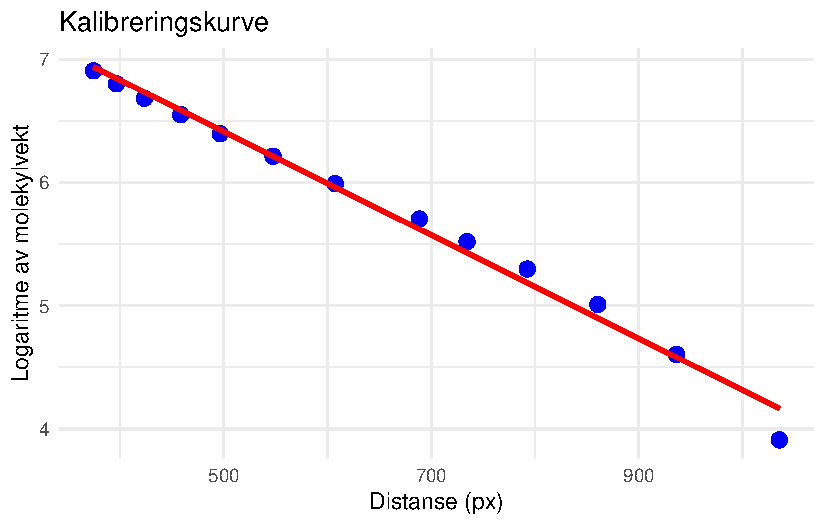
\includegraphics{02-regression-models_files/figure-pdf/fig-fig2-1.pdf}

}

\caption{\label{fig-fig2}}

\end{figure}%

\newpage

\begingroup\fontsize{10}{12}\selectfont

\begin{longtable}[t]{>{}c>{}c>{}c}

\caption{\label{tbl-tbl2}Predikerte molekylvekter for ukjente distanser}

\tabularnewline

\\
\toprule
\cellcolor[HTML]{404080}{\textcolor{white}{\textbf{Båndnummer}}} & \cellcolor[HTML]{404080}{\textcolor{white}{\textbf{Distanse (px)}}} & \cellcolor[HTML]{404080}{\textcolor{white}{\textbf{Predikert molekylvekt (bp)}}}\\
\midrule
\textbf{\cellcolor{gray!10}{1}} & \cellcolor[HTML]{F0F0FF}{\cellcolor{gray!10}{1208.5}} & \cellcolor[HTML]{F0F0FF}{\cellcolor{gray!10}{\cellcolor{red!25}31.22}}\\
\textbf{2} & \cellcolor[HTML]{F0F0FF}{600.5} & \cellcolor[HTML]{F0F0FF}{\cellcolor{yellow!25}400.05}\\
\textbf{\cellcolor{gray!10}{3}} & \cellcolor[HTML]{F0F0FF}{\cellcolor{gray!10}{18.5}} & \cellcolor[HTML]{F0F0FF}{\cellcolor{gray!10}{\cellcolor{green!25}4595.75}}\\
\textbf{4} & \cellcolor[HTML]{F0F0FF}{383.5} & \cellcolor[HTML]{F0F0FF}{\cellcolor{green!25}994.09}\\
\textbf{\cellcolor{gray!10}{5}} & \cellcolor[HTML]{F0F0FF}{\cellcolor{gray!10}{408.5}} & \cellcolor[HTML]{F0F0FF}{\cellcolor{gray!10}{\cellcolor{green!25}895.12}}\\
\addlinespace
\textbf{6} & \cellcolor[HTML]{F0F0FF}{436.5} & \cellcolor[HTML]{F0F0FF}{\cellcolor{green!25}795.93}\\
\textbf{\cellcolor{gray!10}{7}} & \cellcolor[HTML]{F0F0FF}{\cellcolor{gray!10}{470.5}} & \cellcolor[HTML]{F0F0FF}{\cellcolor{gray!10}{\cellcolor{green!25}690.14}}\\
\textbf{8} & \cellcolor[HTML]{F0F0FF}{508.5} & \cellcolor[HTML]{F0F0FF}{\cellcolor{green!25}588.45}\\
\textbf{\cellcolor{gray!10}{9}} & \cellcolor[HTML]{F0F0FF}{\cellcolor{gray!10}{559.5}} & \cellcolor[HTML]{F0F0FF}{\cellcolor{gray!10}{\cellcolor{yellow!25}475.12}}\\
\textbf{10} & \cellcolor[HTML]{F0F0FF}{618.5} & \cellcolor[HTML]{F0F0FF}{\cellcolor{yellow!25}370.95}\\
\addlinespace
\textbf{\cellcolor{gray!10}{11}} & \cellcolor[HTML]{F0F0FF}{\cellcolor{gray!10}{696.5}} & \cellcolor[HTML]{F0F0FF}{\cellcolor{gray!10}{\cellcolor{yellow!25}267.44}}\\
\textbf{12} & \cellcolor[HTML]{F0F0FF}{742.5} & \cellcolor[HTML]{F0F0FF}{\cellcolor{yellow!25}220.51}\\
\textbf{\cellcolor{gray!10}{13}} & \cellcolor[HTML]{F0F0FF}{\cellcolor{gray!10}{798.5}} & \cellcolor[HTML]{F0F0FF}{\cellcolor{gray!10}{\cellcolor{yellow!25}174.34}}\\
\textbf{14} & \cellcolor[HTML]{F0F0FF}{862.5} & \cellcolor[HTML]{F0F0FF}{\cellcolor{yellow!25}133.3}\\
\textbf{\cellcolor{gray!10}{15}} & \cellcolor[HTML]{F0F0FF}{\cellcolor{gray!10}{935.5}} & \cellcolor[HTML]{F0F0FF}{\cellcolor{gray!10}{\cellcolor{red!25}98.14}}\\
\addlinespace
\textbf{16} & \cellcolor[HTML]{F0F0FF}{993.5} & \cellcolor[HTML]{F0F0FF}{\cellcolor{red!25}76.94}\\
\bottomrule

\end{longtable}

\endgroup{}

\subsection{Diskusjon}\label{diskusjon-2}

I denne delen av oppgaven har vi benyttet en kalibreringskurve for å
predikere størrelsene på ukjente DNA-fragmenter fra en
agarosegelelektroforese. Ved å bruke et kjent DNA-ladder med kjente
molekylvekter, etablerte vi en lineær sammenheng mellom logaritmen av
molekylvekten og migrasjonsavstanden på gelen.

Resultatene viser en tydelig lineær korrelasjon mellom log(mw) og
distanse, noe som er i tråd med teori, da mindre DNA-fragmenter migrerer
lenger gjennom gelen enn større fragmenter. Den tilpassede lineære
modellen ble deretter brukt til å estimere molekylvektene til de ukjente
fragmentene basert på deres migrasjonsavstander (Figure~\ref{fig-fig2}).

Tabellen presenterer de predikerte molekylvektene for hvert ukjent bånd,
og fargekodingen gir en visuell indikasjon på fragmentenes relative
størrelser (Table~\ref{tbl-tbl2}). Dette er nyttig for raskt å
identifisere fragmenter av interesse, spesielt i komplekse prøver med
mange bånd.

Det er viktig å være oppmerksom på at nøyaktigheten av prediksjonene
avhenger av flere faktorer. Kvaliteten på gelen, nøyaktigheten i måling
av migrasjonsavstander, og lineariteten i området av molekylvekter som
analyseres, kan alle påvirke resultatene. For eksempel kan avvik i
gelens konsistens eller løpeforhold føre til uregelmessig migrasjon av
DNA-fragmenter, noe som kan gi feilaktige estimater.

Videre antar den lineære modellen en eksponentiell sammenheng mellom
migrasjonsavstand og molekylvekt, noe som kan være mindre nøyaktig for
svært store eller små fragmenter. I slike tilfeller kan det være
fordelaktig å bruke en ikke-lineær modell eller å inkludere flere
kalibreringspunkter for å forbedre presisjonen.

Samlet sett demonstrerer denne analysen effektiviteten av å bruke
gelelektroforese kombinert med kalibreringskurver for å estimere
størrelsen på ukjente DNA-fragmenter. Dette er en grunnleggende teknikk
i molekylærbiologi som er essensiell for en rekke applikasjoner,
inkludert genotyping, kloning og diagnostikk.

\section{Part 3 - Interpreting a regression
table}\label{part-3---interpreting-a-regression-table}

\subsection{Metode}\label{metode-3}

I denne analysen undersøkte vi sammenhengen mellom treningsalder (antall
år med trening) og testosteronkonsentrasjon i blodet ved tidspunkt T1
(målt i ng \textbf{×} dl-1). Vi benyttet datasettet hypertrophy fra
exscidata-pakken i R. Variablene som ble analysert var TRAINING\_AGE
(treningsalder) og TESTOSTERONE\_T1 (testosteronnivå ved T1).

En enkel lineær regresjonsanalyse ble utført med testosteronnivå som
avhengig variabel og treningsalder som uavhengig variabel.
Regresjonsmodellen ble tilpasset ved hjelp av funksjonen lm() i R:

m \textless- lm(TESTOSTERONE\_T1 \textasciitilde{} TRAINING\_AGE, data =
dat) Vi hentet ut regresjonskoeffisientene, standardfeilen, t-verdien og
p-verdien fra modellens sammendrag ved hjelp av summary()-funksjonen. Vi
estimerte også det forventede testosteronnivået etter 10 år med trening
ved å bruke regresjonsligningen.

\subsection{Resultat}\label{resultat-3}

\begin{figure}

\centering{

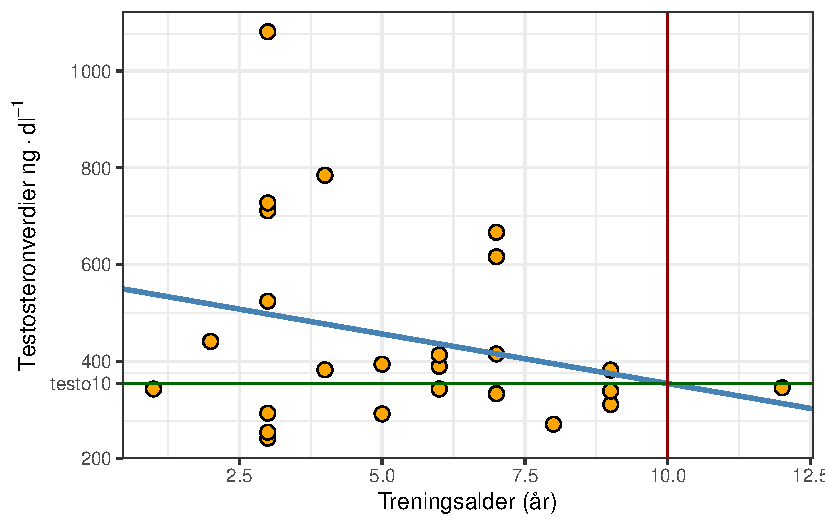
\includegraphics{02-regression-models_files/figure-pdf/fig-fig3-1.pdf}

}

\caption{\label{fig-fig3}Figur 3: Sammenheng mellom treningsalder og
testosteronverdier i blodet}

\end{figure}%

Den lineære regresjonsmodellen viste at det var en negativ sammenheng
mellom treningsalder og testosteronkonsentrasjon i blodet
(Figure~\ref{fig-fig3}). Regresjonskoeffisienten for treningsalder var
-20.51ng \textbf{×} dl-1 per år, noe som indikerer at testosteronnivået
synker med gjennomsnittlig 20.51ng \textbf{×} dl-1 for hvert år med
trening. Interceptet i modellen var 559.36ng \textbf{×} dl-1, som
representerer det estimerte testosteronnivået for en person uten
treningserfaring.

T-verdien for koeffisienten var -1.39, og tilhørende p-verdi var 0.178.
Siden p-verdien er høyere enn signifikansnivået på 0,05, er sammenhengen
ikke statistisk signifikant. Dette betyr at vi ikke har tilstrekkelig
bevis til å konkludere med at det er en lineær sammenheng mellom
treningsalder og testosteronnivå i denne populasjonen.

Ved å bruke regresjonsligningen estimerte vi testosteronnivået etter 10
år med trening til å være 354.26ng \textbf{×} dl-1. Dette ble beregnet
ved å sette inn TRAINING\_AGE = 10 i modellen.

Dette estimatet illustrerer den forventede nedgangen i testosteronnivå
basert på modellen, men gitt den ikke-signifikante p-verdien bør
resultatene tolkes med forsiktighet.

\subsection{Diskusjon}\label{diskusjon-3}

Fra datasettet hypertrophy valgte vi å se på sammenhengen mellom
testosteronkonsentrasjon i blodet (ng \textbf{×} dl-1) og treningsalder
(antall år med trening). Den lineære modellen forteller at
testosteronkonsentrasjonen i blodet synker med 20.51 ng \textbf{×} dl-1
for hvert treningsår. Etter 10 år med trening, estimerer den lineære
modellen et testosteronnivå på 354.26 ng \textbf{×} dl-1.

Analysen av dataene viser en p-verdi på 0.178, noe som indikerer at det
ikke er statistisk signifikant bevis for en sammenheng mellom
treningsalder og nivået av testosteron i blodet. Siden p-verdien er
høyere enn det vanlige signifikansnivået på 0,05, kan vi ikke avvise
nullhypotesen, som antyder at det ikke er noen betydelig effekt eller
sammenheng mellom de to variablene i dette datasettet. Dette betyr at
variasjonen i testosteronnivåer ikke ser ut til å være relatert til hvor
lenge individene har trent.

I analysen av sammenhengen mellom treningsalder og testosteronnivåer i
blodet ses det en t-verdi på -1.39. Den høye t-verdien på -1.39, og en
p-verdi på 0.178. Denne p-verdien er høyere enn det vanlige
signifikansnivået på 0,05, noe som betyr at vi ikke har tilstrekkelig
statistisk bevis for å avvise nullhypotesen. Selv om t-verdien indikerer
en mulig sammenheng mellom treningsalder og testosteronnivå, er det ikke
nok evidens til å konkludere med at denne sammenhengen er signifikant.
Dermed kan vi konkludere med at selv om det kan være en tendens til en
sammenheng mellom treningsalder og testosteronnivåer, er resultatene fra
denne analysen ikke sterke nok til å si at treningsalder har en reell
effekt på testosteronnivåene i blodet.

\bookmarksetup{startatroot}

\chapter{Å trekke slutninger fra statistiske modeller og statistisk
styrke}\label{uxe5-trekke-slutninger-fra-statistiske-modeller-og-statistisk-styrke}

\section{Spørsmål og svar}\label{spuxf8rsmuxe5l-og-svar}

\subsection{Estimate}\label{estimate}

Et \textbf{estimat} er en verdi vi får ved å anvende en lineær modell på
våre data. Dette tallet representerer vår beste gjetning av den sanne
verdien til parameteren vi ønsker å estimere i populasjonen, basert på
vårt utvalg. I konteksten av en regresjonsanalyse er dette ofte
regresjonskoeffisienten, som estimerer sammenhengen mellom en uavhengig
variabel og den avhengige variabelen \emph{y}.

\textbf{Standardfeilen} (SE) kvantifiserer usikkerheten knyttet til
estimatet vårt. Den måler den forventede variasjonen i estimatet dersom
vi skulle trekke mange utvalg fra populasjonen og beregne estimatet hver
gang. Med andre ord er standardfeilen standardavviket til estimatets
utvalgsfordeling, og indikerer hvor mye estimatet vårt potensielt kan
variere fra utvalg til utvalg på grunn av tilfeldig sampling.

\textbf{t-verdien} er forholdet mellom estimatet og standardfeilen
(\(t = \frac{{estimat}}{{SE}}\)). Den indikerer hvor mange standardfeil
estimatet er unna null\textsuperscript{2}. En høy absolutt t-verdi tyder
på at estimatet er signifikant forskjellig fra null.

\textbf{P-verdien} angir sannsynligheten for å observere en t-verdi som
er minst like ekstrem som den vi har fått, gitt at nullhypotesen er
sann. Det vil si, den måler sannsynligheten for å få våre data, eller
data som er mer ekstreme, dersom det faktisk ikke er noen effekt (dvs.
hvis den sanne parameteren er null). En lav p-verdi indikerer at et så
ekstremt resultat er lite sannsynlig under nullhypotesen, noe som gir
grunnlag for å forkaste nullhypotesen\textsuperscript{2}.

I vårt tilfelle har vi en høy p-verdi, noe som indikerer at vi ikke kan
forkaste nullhypotesen. Dette betyr at det ikke er tilstrekkelig bevis
til å konkludere med at det er en signifikant forskjell fra null.

\subsection{m1 vs m2}\label{m1-vs-m2}

Forskjellen mellom studiene kommer fra størrelsen på utvalget som er
brukt i de to forskjellige. I \emph{m1} er det brukt ett mye mindre
utvalg, noe som fører til større usikkerhet rundt resultatene. I
\emph{m2} er det brukt et større utvalg, som gjør at det estimerte
gjennomsnittet blir nærmere populasjonsgjennomsnittet og standardfeilen
blir dermed mindre. Dette gir i vårt tilfelle en høyere \textbf{t-verdi}
og en lavere \textbf{p-verdi}\textsuperscript{2}.

\subsection{Shaded areas}\label{shaded-areas}

Vi bruker de grå feltene for å vise de ekstreme verdiene vi har fra
testen vår. Jo lenger ut i halene vi kommer, desto større sannsynlighet
er det for at dette er et uvanlig resultat å se.

\subsection{\texorpdfstring{Standard deviation of \textbf{estimate} and
avg. \textbf{se} for each
study.}{Standard deviation of estimate and avg. se for each study.}}\label{standard-deviation-of-estimate-and-avg.-se-for-each-study.}

Standard deviation for modellen med 8 i population er 1.07, mens det for
modellen med 40 i population er 0.48. Når det kommer til gjennomsnittlig
standardfeil ligger den på 1.02 for modellen med 8 i population, mens
den for modellen med 40 i population ligger på 0.47. Grunnen til at
tallene er såpass like som de er for \textbf{SD} og \textbf{avg se} er
at begge beregningene er mål på variasjon. I denne sammenhengen er
standardfeilen et mål på hvor mye gjennomsnittet avviker fra det sanne
populasjonsgjennomsnittet.

\subsection{P-value histogram}\label{p-value-histogram}

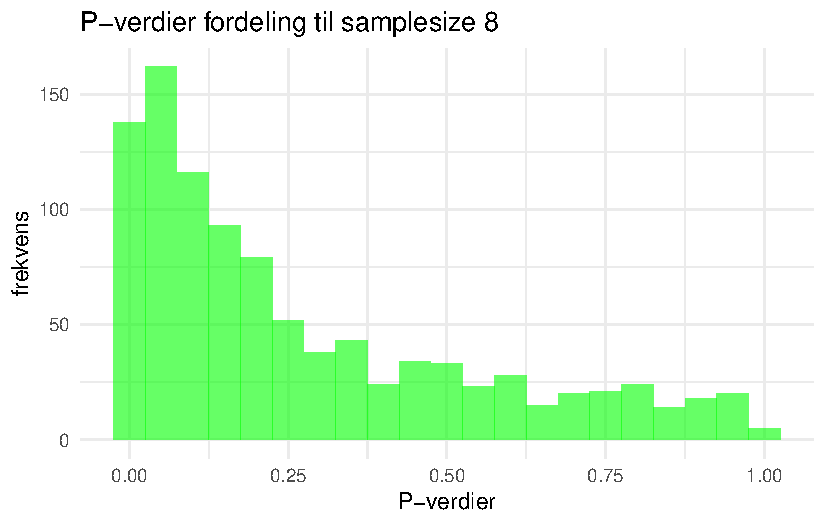
\includegraphics{03-statistical-inference_files/figure-pdf/P-verdi histogram SS8-1.pdf}

Når vi ser histogrammet for modellen med utvalgsstørrelse på 8, ser vi
tydelig at det er mange observasjoner av høye p-verdier. Dette
gjenspeiler den lave statistiske poweren vi får av å gjøre studier med
en så liten utvalgsstørrelse.

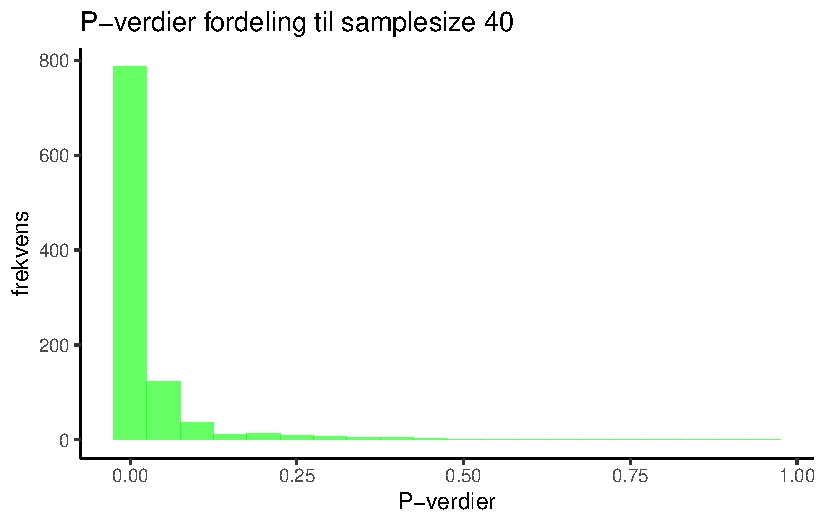
\includegraphics{03-statistical-inference_files/figure-pdf/P-verdi histogram SS40-1.pdf}

På histogrammet med utvalgsstørrelse på 40 ser vi at det er en mye
større samling av observasjoner på lave p-verdier. Dette gjenspeiler det
vi vet om at en større utvalgsstørrelse gir en større statistisk power.

\subsection{Antall studier med statistisk
signifikans}\label{antall-studier-med-statistisk-signifikans}

I studiene med utvalgsstørrelse på 8 ser vi at det er 227 studier som
viser statistisk signifikans, mens det i studiene med utvalgsstørrelse
på 40 er hele 865 studier som viser statistisk signifikans. Dette gir et
godt bilde på hvor mye utvalgsstørrelsen har å si for resultatet i
utregningen vår. I mitt tilfelle har jeg valgt å sette terskelen for
signifikans (p-verdi) til 0.05.

\subsection{Power of a one-sample
t-test}\label{power-of-a-one-sample-t-test}

Når vi gjennomfører utregningen ser vi at studiene med lav
utvalgsstørrelse (8) får en mye lavere statistisk styrke (0.232) enn
studiene med utvalgsstørrelse på 40 (0.869). Svarene vi får av disse
utregningene støtter det vi tidligere har funnet ut, at dersom vi har et
større utvalg, er det større sannsynlighet for at vi ser en faktisk
effekt, og at det ikke er en tilfeldighet at vi har funnet det vi har i
studien. I dette tilfelle vil vi da få en 86.9\% sjanse for å oppdage en
sann effekt.

\subsection{Med signifikansnivå på 0.05 hvor mange studier gir ``falsk
positiv'' ved gjennomføring av mange repeterte
studier?}\label{med-signifikansnivuxe5-puxe5-0.05-hvor-mange-studier-gir-falsk-positiv-ved-gjennomfuxf8ring-av-mange-repeterte-studier}

Ved å gjøre 1000 repeterte studier, vil vi få omtrent 50 falske positive
hvis vi setter signifikansnivået til 0.05. I min utregning fikk jeg da
49 for studiene med utvalgsstørrelse på 8 og 59 på studiene med
utvalgsstørrelse 40. Om jeg endrer signifikansnivået og setter alpha
enda lavere vil resultatet endre seg litt. Med en signifikansverdi på
0.025 vil det i studiene med utvalgsstørrelse 8 gi meg 30 falske
positive, mens det på studiene med 40 i utvalgsstørrelse gir 22 falske
positive.

\section{Code-chunks fra topp til
bunn}\label{code-chunks-fra-topp-til-bunn}

\begin{Shaded}
\begin{Highlighting}[]
\FunctionTok{set.seed}\NormalTok{(}\DecValTok{1}\NormalTok{)}
\NormalTok{population }\OtherTok{\textless{}{-}} \FunctionTok{rnorm}\NormalTok{(}\DecValTok{1000000}\NormalTok{, }\AttributeTok{mean =} \FloatTok{1.5}\NormalTok{, }\AttributeTok{sd =} \DecValTok{3}\NormalTok{)}

\NormalTok{samp1 }\OtherTok{\textless{}{-}} \FunctionTok{data.frame}\NormalTok{(}\AttributeTok{y =} \FunctionTok{sample}\NormalTok{(population, }\DecValTok{8}\NormalTok{, }\AttributeTok{replace =} \ConstantTok{FALSE}\NormalTok{))}
\NormalTok{samp2 }\OtherTok{\textless{}{-}} \FunctionTok{data.frame}\NormalTok{(}\AttributeTok{y =} \FunctionTok{sample}\NormalTok{(population, }\DecValTok{40}\NormalTok{, }\AttributeTok{replace =} \ConstantTok{FALSE}\NormalTok{))}

\NormalTok{m1 }\OtherTok{\textless{}{-}} \FunctionTok{lm}\NormalTok{(y }\SpecialCharTok{\textasciitilde{}} \DecValTok{1}\NormalTok{, }\AttributeTok{data =}\NormalTok{ samp1)}
\NormalTok{m2 }\OtherTok{\textless{}{-}} \FunctionTok{lm}\NormalTok{(y }\SpecialCharTok{\textasciitilde{}} \DecValTok{1}\NormalTok{, }\AttributeTok{data =}\NormalTok{ samp2)}

\CommentTok{\# Skjul summary{-}output}
\FunctionTok{invisible}\NormalTok{(}\FunctionTok{summary}\NormalTok{(m1))}
\FunctionTok{invisible}\NormalTok{(}\FunctionTok{summary}\NormalTok{(m2))}
\end{Highlighting}
\end{Shaded}

\begin{Shaded}
\begin{Highlighting}[]
\CommentTok{\# Create data frames to store the model estimates}
\NormalTok{results\_8 }\OtherTok{\textless{}{-}} \FunctionTok{data.frame}\NormalTok{(}\AttributeTok{estimate =} \FunctionTok{rep}\NormalTok{(}\ConstantTok{NA}\NormalTok{, }\DecValTok{1000}\NormalTok{), }
                      \AttributeTok{se =} \FunctionTok{rep}\NormalTok{(}\ConstantTok{NA}\NormalTok{, }\DecValTok{1000}\NormalTok{), }
                      \AttributeTok{pval =} \FunctionTok{rep}\NormalTok{(}\ConstantTok{NA}\NormalTok{, }\DecValTok{1000}\NormalTok{), }
                      \AttributeTok{n =} \DecValTok{8}\NormalTok{)  }

\NormalTok{results\_40 }\OtherTok{\textless{}{-}} \FunctionTok{data.frame}\NormalTok{(}\AttributeTok{estimate =} \FunctionTok{rep}\NormalTok{(}\ConstantTok{NA}\NormalTok{, }\DecValTok{1000}\NormalTok{), }
                      \AttributeTok{se =} \FunctionTok{rep}\NormalTok{(}\ConstantTok{NA}\NormalTok{, }\DecValTok{1000}\NormalTok{), }
                      \AttributeTok{pval =} \FunctionTok{rep}\NormalTok{(}\ConstantTok{NA}\NormalTok{, }\DecValTok{1000}\NormalTok{), }
                      \AttributeTok{n =} \DecValTok{40}\NormalTok{)}

\CommentTok{\# A for loop used to sample 1000 studies, each iteration (i) will draw a new sample}
\CommentTok{\# from the population. }

\ControlFlowTok{for}\NormalTok{(i }\ControlFlowTok{in} \DecValTok{1}\SpecialCharTok{:}\DecValTok{1000}\NormalTok{) \{}
  
  \CommentTok{\# Draw a sample }
\NormalTok{  samp1 }\OtherTok{\textless{}{-}} \FunctionTok{data.frame}\NormalTok{(}\AttributeTok{y =} \FunctionTok{sample}\NormalTok{(population, }\DecValTok{8}\NormalTok{, }\AttributeTok{replace =} \ConstantTok{FALSE}\NormalTok{))}
\NormalTok{  samp2 }\OtherTok{\textless{}{-}} \FunctionTok{data.frame}\NormalTok{(}\AttributeTok{y =} \FunctionTok{sample}\NormalTok{(population, }\DecValTok{40}\NormalTok{, }\AttributeTok{replace =} \ConstantTok{FALSE}\NormalTok{))}

  \CommentTok{\# Model the data}
\NormalTok{  m1 }\OtherTok{\textless{}{-}} \FunctionTok{lm}\NormalTok{(y }\SpecialCharTok{\textasciitilde{}} \DecValTok{1}\NormalTok{, }\AttributeTok{data =}\NormalTok{ samp1)}
\NormalTok{  m2 }\OtherTok{\textless{}{-}} \FunctionTok{lm}\NormalTok{(y }\SpecialCharTok{\textasciitilde{}} \DecValTok{1}\NormalTok{, }\AttributeTok{data =}\NormalTok{ samp2)}
  
  \CommentTok{\# Extract values from the models}
\NormalTok{  results\_8[i, }\DecValTok{1}\NormalTok{] }\OtherTok{\textless{}{-}} \FunctionTok{coef}\NormalTok{(}\FunctionTok{summary}\NormalTok{(m1))[}\DecValTok{1}\NormalTok{, }\DecValTok{1}\NormalTok{]}
\NormalTok{  results\_8[i, }\DecValTok{2}\NormalTok{] }\OtherTok{\textless{}{-}} \FunctionTok{coef}\NormalTok{(}\FunctionTok{summary}\NormalTok{(m1))[}\DecValTok{1}\NormalTok{, }\DecValTok{2}\NormalTok{]}
\NormalTok{  results\_8[i, }\DecValTok{3}\NormalTok{] }\OtherTok{\textless{}{-}} \FunctionTok{coef}\NormalTok{(}\FunctionTok{summary}\NormalTok{(m1))[}\DecValTok{1}\NormalTok{, }\DecValTok{4}\NormalTok{]}

\NormalTok{  results\_40[i, }\DecValTok{1}\NormalTok{] }\OtherTok{\textless{}{-}} \FunctionTok{coef}\NormalTok{(}\FunctionTok{summary}\NormalTok{(m2))[}\DecValTok{1}\NormalTok{, }\DecValTok{1}\NormalTok{]}
\NormalTok{  results\_40[i, }\DecValTok{2}\NormalTok{] }\OtherTok{\textless{}{-}} \FunctionTok{coef}\NormalTok{(}\FunctionTok{summary}\NormalTok{(m2))[}\DecValTok{1}\NormalTok{, }\DecValTok{2}\NormalTok{]}
\NormalTok{  results\_40[i, }\DecValTok{3}\NormalTok{] }\OtherTok{\textless{}{-}} \FunctionTok{coef}\NormalTok{(}\FunctionTok{summary}\NormalTok{(m2))[}\DecValTok{1}\NormalTok{, }\DecValTok{4}\NormalTok{]}
  
  
\NormalTok{\}}


\CommentTok{\# Save the results in a combined data frame}

\NormalTok{results }\OtherTok{\textless{}{-}} \FunctionTok{bind\_rows}\NormalTok{(results\_8, results\_40)}

\CommentTok{\# Calculate standard deviation of the estimate and the average of the standard error (se)}
\NormalTok{results\_summary }\OtherTok{\textless{}{-}}\NormalTok{ results }\SpecialCharTok{|\textgreater{}} 
  \FunctionTok{group\_by}\NormalTok{(n) }\SpecialCharTok{|\textgreater{}} 
  \FunctionTok{summarise}\NormalTok{(}
    \AttributeTok{sd\_estimate =} \FunctionTok{sd}\NormalTok{(estimate),}
    \AttributeTok{avg\_se =} \FunctionTok{mean}\NormalTok{(se)}
\NormalTok{  )}


\NormalTok{sd\_est\_8 }\OtherTok{\textless{}{-}} \FunctionTok{sd}\NormalTok{(results}\SpecialCharTok{$}\NormalTok{estimate[results}\SpecialCharTok{$}\NormalTok{n }\SpecialCharTok{==} \DecValTok{8}\NormalTok{])}
\NormalTok{avg\_se\_8 }\OtherTok{\textless{}{-}} \FunctionTok{mean}\NormalTok{(results}\SpecialCharTok{$}\NormalTok{se[results}\SpecialCharTok{$}\NormalTok{n }\SpecialCharTok{==} \DecValTok{8}\NormalTok{])}

\NormalTok{sd\_est\_40 }\OtherTok{\textless{}{-}} \FunctionTok{sd}\NormalTok{(results}\SpecialCharTok{$}\NormalTok{estimate[results}\SpecialCharTok{$}\NormalTok{n }\SpecialCharTok{==} \DecValTok{40}\NormalTok{])}
\NormalTok{avg\_se\_40 }\OtherTok{\textless{}{-}} \FunctionTok{mean}\NormalTok{(results}\SpecialCharTok{$}\NormalTok{se[results}\SpecialCharTok{$}\NormalTok{n }\SpecialCharTok{==} \DecValTok{40}\NormalTok{])}

\NormalTok{rounded\_sd\_est\_8 }\OtherTok{\textless{}{-}} \FunctionTok{round}\NormalTok{(sd\_est\_8, }\DecValTok{2}\NormalTok{)}
\NormalTok{rounded\_avg\_se\_8 }\OtherTok{\textless{}{-}} \FunctionTok{round}\NormalTok{(avg\_se\_8, }\DecValTok{2}\NormalTok{)}
\NormalTok{rounded\_sd\_est\_40 }\OtherTok{\textless{}{-}} \FunctionTok{round}\NormalTok{(sd\_est\_40, }\DecValTok{2}\NormalTok{)}
\NormalTok{rounded\_avg\_se\_40 }\OtherTok{\textless{}{-}} \FunctionTok{round}\NormalTok{(avg\_se\_40, }\DecValTok{2}\NormalTok{)}
\end{Highlighting}
\end{Shaded}

\begin{Shaded}
\begin{Highlighting}[]
\FunctionTok{ggplot}\NormalTok{(results[results}\SpecialCharTok{$}\NormalTok{n }\SpecialCharTok{==} \DecValTok{8}\NormalTok{, ], }\FunctionTok{aes}\NormalTok{(}\AttributeTok{x =}\NormalTok{ pval)) }\SpecialCharTok{+}
  \FunctionTok{geom\_histogram}\NormalTok{(}\AttributeTok{binwidth =} \FloatTok{0.05}\NormalTok{, }\AttributeTok{fill =} \StringTok{"green"}\NormalTok{, }\AttributeTok{alpha =} \FloatTok{0.6}\NormalTok{) }\SpecialCharTok{+}
  \FunctionTok{labs}\NormalTok{(}\AttributeTok{title =} \StringTok{"P{-}verdier fordeling til samplesize 8"}\NormalTok{,}
       \AttributeTok{x =} \StringTok{"P{-}verdier"}\NormalTok{,}
       \AttributeTok{y =} \StringTok{"frekvens"}\NormalTok{) }\SpecialCharTok{+}
  \FunctionTok{theme\_minimal}\NormalTok{()}
\end{Highlighting}
\end{Shaded}

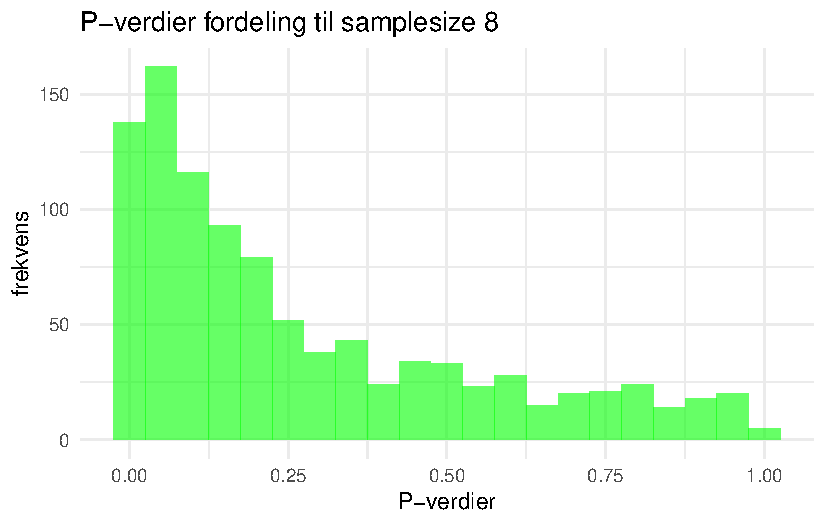
\includegraphics{03-statistical-inference_files/figure-pdf/Kode 3-1.pdf}

\begin{Shaded}
\begin{Highlighting}[]
\NormalTok{alpha }\OtherTok{\textless{}{-}} \FloatTok{0.05}

\NormalTok{significant\_8 }\OtherTok{\textless{}{-}} \FunctionTok{sum}\NormalTok{(results}\SpecialCharTok{$}\NormalTok{pval[results}\SpecialCharTok{$}\NormalTok{n }\SpecialCharTok{==} \DecValTok{8}\NormalTok{] }\SpecialCharTok{\textless{}}\NormalTok{ alpha)}
\NormalTok{significant\_40 }\OtherTok{\textless{}{-}} \FunctionTok{sum}\NormalTok{(results}\SpecialCharTok{$}\NormalTok{pval[results}\SpecialCharTok{$}\NormalTok{n }\SpecialCharTok{==} \DecValTok{40}\NormalTok{] }\SpecialCharTok{\textless{}}\NormalTok{ alpha)}
\end{Highlighting}
\end{Shaded}

\begin{Shaded}
\begin{Highlighting}[]
\NormalTok{effect\_size }\OtherTok{\textless{}{-}} \FloatTok{1.5} \SpecialCharTok{/} \DecValTok{3}

\NormalTok{power\_8 }\OtherTok{\textless{}{-}} \FunctionTok{pwr.t.test}\NormalTok{(}\AttributeTok{n =} \DecValTok{8}\NormalTok{,}
                      \AttributeTok{d =}\NormalTok{ effect\_size,}
                      \AttributeTok{sig.level =}\NormalTok{ alpha,}
                      \AttributeTok{type =} \StringTok{"one.sample"}\NormalTok{)}\SpecialCharTok{$}\NormalTok{power}
\NormalTok{rounded\_power\_8 }\OtherTok{\textless{}{-}} \FunctionTok{round}\NormalTok{(power\_8, }\DecValTok{3}\NormalTok{)}


\NormalTok{power\_40 }\OtherTok{\textless{}{-}} \FunctionTok{pwr.t.test}\NormalTok{(}\AttributeTok{n =} \DecValTok{40}\NormalTok{,}
                       \AttributeTok{d =}\NormalTok{ effect\_size,}
                       \AttributeTok{sig.level =}\NormalTok{ alpha,}
                       \AttributeTok{type =} \StringTok{"one.sample"}\NormalTok{)}\SpecialCharTok{$}\NormalTok{power}

\NormalTok{rounded\_power\_40 }\OtherTok{\textless{}{-}} \FunctionTok{round}\NormalTok{(power\_40, }\DecValTok{3}\NormalTok{)}

\NormalTok{rounded\_power\_40\_perc }\OtherTok{\textless{}{-}}\NormalTok{ rounded\_power\_40 }\SpecialCharTok{*} \DecValTok{100}
\end{Highlighting}
\end{Shaded}

\begin{Shaded}
\begin{Highlighting}[]
\FunctionTok{set.seed}\NormalTok{(}\DecValTok{1}\NormalTok{)}
\NormalTok{population }\OtherTok{\textless{}{-}} \FunctionTok{rnorm}\NormalTok{(}\DecValTok{1000000}\NormalTok{, }\AttributeTok{mean =} \DecValTok{0}\NormalTok{, }\AttributeTok{sd =} \DecValTok{3}\NormalTok{)}


\CommentTok{\# Create data frames to store the model estimates}
\NormalTok{results\_8 }\OtherTok{\textless{}{-}} \FunctionTok{data.frame}\NormalTok{(}\AttributeTok{estimate =} \FunctionTok{rep}\NormalTok{(}\ConstantTok{NA}\NormalTok{, }\DecValTok{1000}\NormalTok{), }
                      \AttributeTok{se =} \FunctionTok{rep}\NormalTok{(}\ConstantTok{NA}\NormalTok{, }\DecValTok{1000}\NormalTok{), }
                      \AttributeTok{pval =} \FunctionTok{rep}\NormalTok{(}\ConstantTok{NA}\NormalTok{, }\DecValTok{1000}\NormalTok{), }
                      \AttributeTok{n =} \DecValTok{8}\NormalTok{)  }

\NormalTok{results\_40 }\OtherTok{\textless{}{-}} \FunctionTok{data.frame}\NormalTok{(}\AttributeTok{estimate =} \FunctionTok{rep}\NormalTok{(}\ConstantTok{NA}\NormalTok{, }\DecValTok{1000}\NormalTok{), }
                      \AttributeTok{se =} \FunctionTok{rep}\NormalTok{(}\ConstantTok{NA}\NormalTok{, }\DecValTok{1000}\NormalTok{), }
                      \AttributeTok{pval =} \FunctionTok{rep}\NormalTok{(}\ConstantTok{NA}\NormalTok{, }\DecValTok{1000}\NormalTok{), }
                      \AttributeTok{n =} \DecValTok{40}\NormalTok{)}

\CommentTok{\# A for loop used to sample 1000 studies, each iteration (i) will draw a new sample}
\CommentTok{\# from the population. }

\ControlFlowTok{for}\NormalTok{(i }\ControlFlowTok{in} \DecValTok{1}\SpecialCharTok{:}\DecValTok{1000}\NormalTok{) \{}
  
  \CommentTok{\# Draw a sample }
\NormalTok{  samp1 }\OtherTok{\textless{}{-}} \FunctionTok{data.frame}\NormalTok{(}\AttributeTok{y =} \FunctionTok{sample}\NormalTok{(population, }\DecValTok{8}\NormalTok{, }\AttributeTok{replace =} \ConstantTok{FALSE}\NormalTok{))}
\NormalTok{  samp2 }\OtherTok{\textless{}{-}} \FunctionTok{data.frame}\NormalTok{(}\AttributeTok{y =} \FunctionTok{sample}\NormalTok{(population, }\DecValTok{40}\NormalTok{, }\AttributeTok{replace =} \ConstantTok{FALSE}\NormalTok{))}

  \CommentTok{\# Model the data}
\NormalTok{  m1 }\OtherTok{\textless{}{-}} \FunctionTok{lm}\NormalTok{(y }\SpecialCharTok{\textasciitilde{}} \DecValTok{1}\NormalTok{, }\AttributeTok{data =}\NormalTok{ samp1)}
\NormalTok{  m2 }\OtherTok{\textless{}{-}} \FunctionTok{lm}\NormalTok{(y }\SpecialCharTok{\textasciitilde{}} \DecValTok{1}\NormalTok{, }\AttributeTok{data =}\NormalTok{ samp2)}
  
  \CommentTok{\# Extract values from the models}
\NormalTok{  results\_8[i, }\DecValTok{1}\NormalTok{] }\OtherTok{\textless{}{-}} \FunctionTok{coef}\NormalTok{(}\FunctionTok{summary}\NormalTok{(m1))[}\DecValTok{1}\NormalTok{, }\DecValTok{1}\NormalTok{]}
\NormalTok{  results\_8[i, }\DecValTok{2}\NormalTok{] }\OtherTok{\textless{}{-}} \FunctionTok{coef}\NormalTok{(}\FunctionTok{summary}\NormalTok{(m1))[}\DecValTok{1}\NormalTok{, }\DecValTok{2}\NormalTok{]}
\NormalTok{  results\_8[i, }\DecValTok{3}\NormalTok{] }\OtherTok{\textless{}{-}} \FunctionTok{coef}\NormalTok{(}\FunctionTok{summary}\NormalTok{(m1))[}\DecValTok{1}\NormalTok{, }\DecValTok{4}\NormalTok{]}

\NormalTok{  results\_40[i, }\DecValTok{1}\NormalTok{] }\OtherTok{\textless{}{-}} \FunctionTok{coef}\NormalTok{(}\FunctionTok{summary}\NormalTok{(m2))[}\DecValTok{1}\NormalTok{, }\DecValTok{1}\NormalTok{]}
\NormalTok{  results\_40[i, }\DecValTok{2}\NormalTok{] }\OtherTok{\textless{}{-}} \FunctionTok{coef}\NormalTok{(}\FunctionTok{summary}\NormalTok{(m2))[}\DecValTok{1}\NormalTok{, }\DecValTok{2}\NormalTok{]}
\NormalTok{  results\_40[i, }\DecValTok{3}\NormalTok{] }\OtherTok{\textless{}{-}} \FunctionTok{coef}\NormalTok{(}\FunctionTok{summary}\NormalTok{(m2))[}\DecValTok{1}\NormalTok{, }\DecValTok{4}\NormalTok{]}
  
  
\NormalTok{\}}


\CommentTok{\# Save the results in a combined data frame}

\NormalTok{results\_null }\OtherTok{\textless{}{-}} \FunctionTok{bind\_rows}\NormalTok{(results\_8, results\_40)}
\end{Highlighting}
\end{Shaded}

\begin{Shaded}
\begin{Highlighting}[]
\NormalTok{false\_positive\_8 }\OtherTok{\textless{}{-}} \FunctionTok{sum}\NormalTok{(results\_8}\SpecialCharTok{$}\NormalTok{pval }\SpecialCharTok{\textless{}} \FloatTok{0.05}\NormalTok{)}
\NormalTok{false\_positive\_40 }\OtherTok{\textless{}{-}} \FunctionTok{sum}\NormalTok{(results\_40}\SpecialCharTok{$}\NormalTok{pval }\SpecialCharTok{\textless{}} \FloatTok{0.05}\NormalTok{)}


\NormalTok{false\_positive\_8\_alpha0}\FloatTok{.025} \OtherTok{\textless{}{-}} \FunctionTok{sum}\NormalTok{(results\_8}\SpecialCharTok{$}\NormalTok{pval }\SpecialCharTok{\textless{}} \FloatTok{0.025}\NormalTok{)}
\NormalTok{false\_positive\_40\_alpha0}\FloatTok{.025} \OtherTok{\textless{}{-}} \FunctionTok{sum}\NormalTok{(results\_40}\SpecialCharTok{$}\NormalTok{pval }\SpecialCharTok{\textless{}} \FloatTok{0.025}\NormalTok{)}
\end{Highlighting}
\end{Shaded}

\bookmarksetup{startatroot}

\chapter{Studiedesign}\label{studiedesign}

\section{Introduksjon}\label{introduksjon-2}

Formålet med denne sammenligningen er å undersøke ulikheter i de
metodiske valgene blant ulike studier som ser på effekten av
blokkperiodisering av utholdenhetstrening sammenlignet med tradisjonell
utholdenhetstrening på maksimal oksygenopptak (\(\dot{V}O_{2maks}\)).
Videre vil jeg vurdere styrker og svakheter ved studiedesign,
statistiske analyser og resultater. Til slutt vil jeg gi noen
anbefalinger for fremtidige studier.

\section{Metode}\label{metode-4}

Fem ulike studier ble valgt ut, alle med fokus på effekten av
blokkperiodisering av utholdenhetstrening på \(\dot{V}O_{2maks}\).
Studienes styrker og svakheter ble analysert, med spesiell vekt på
studiedesign og statistiske analyser. Studiedesignenes evne til å måle
relevante utfall ble vurdert, samt i hvilken grad de tok hensyn til
eksterne variabler som kunne påvirke resultatene.

\section{Resultat}\label{resultat-4}

Den første studien\textsuperscript{9} brukte et kontrollert design med
objektive målinger som \(\dot{V}O_{2maks}\). Til tross for dette var
utvalgsstørrelsen liten, noe som kan redusere den statistiske kraften og
øke risikoen for type II-feil. Manglende kontroll for eksterne faktorer,
som kosthold og annen fysisk aktivitet utenom studien, kan ha påvirket
resultatene og dermed redusert intern validitet.

Den andre studien\textsuperscript{10} hadde et robust eksperimentelt
design med godt definerte kontrollgrupper og brukte gjentatte målinger
for å spore prestasjonsendringer over tid. Likevel var ekstern validitet
en utfordring på grunn av spesifisiteten til utvalget, som besto av
eliteutøvere. Dette gjør det vanskelig å generalisere funnene til en
bredere befolkning. I tillegg var tidsrammen for studien relativt kort,
noe som begrenser muligheten til å vurdere langsiktige effekter av
treningsintervensjonen.

Studie nummer tre\textsuperscript{11} implementerte blokkperiodisering
og benyttet et bredt spekter av prestasjonsmål. Den korte
intervensjonsperioden og det lave antallet kvinnelige deltakere utgjorde
imidlertid svakheter som kan ha påvirket representativiteten og dermed
generaliserbarheten av konklusjonene. Dette kan også ha ført til
skjevheter i resultatene grunnet kjønnsspesifikke responser på
treningen.

Den fjerde studien\textsuperscript{12} benyttet avanserte statistiske
analyser, inkludert lineære mixed models, og hadde et langsiktig design.
Likevel var utvalgsstørrelsen begrenset, og fokus på eliteutøvere
reduserte generaliserbarheten av funnene til andre populasjoner, slik
som mosjonister eller utøvere på lavere nivåer.

Studie fem\textsuperscript{13} brukte et omfattende design med både
fysiologiske og prestasjonsbaserte utfallsmål. Svakheten var
spesifisiteten til deltakerutvalget, som besto av kvinnelige
eliteutøvere i langrenn. Dette begrenser overførbarheten av resultatene
til mannlige utøvere eller til andre idretter. Det var også behov for en
bedre sammenheng mellom de statistiske testene og forskningsspørsmålene
i studien; for eksempel kunne valg av mer avanserte statistiske metoder
ha gitt dypere innsikt i dataene.

\section{Diskusjon}\label{diskusjon-4}

Studiene har generelt god intern validitet på grunn av robuste
studiedesign og bruk av kontrollgrupper, noe som styrker troverdigheten
til de kausale sammenhengene som blir funnet. Intern validitet refererer
til i hvilken grad studiens resultater faktisk skyldes intervensjonen og
ikke andre faktorer.

Den eksterne validiteten er imidlertid begrenset. Ekstern validitet
handler om i hvilken grad funnene kan generaliseres til andre
populasjoner og kontekster. Små utvalgsstørrelser øker usikkerheten i
estimatene og reduserer statistisk kraft, noe som kan gjøre det
vanskelig å oppdage reelle effekter. Bruk av spesifikke grupper, som
eliteutøvere, betyr at resultatene kanskje ikke er direkte overførbare
til den generelle befolkningen eller til utøvere på lavere nivåer. Dette
skyldes at eliteutøvere kan ha unike fysiologiske egenskaper og
treningsresponser.

Variasjon i varigheten av treningsintervensjonene mellom studiene gjør
det utfordrende å sammenligne resultatene og trekke konklusjoner om
langsiktige effekter. Kortvarige intervensjoner kan mangle tilstrekkelig
tid for å observere betydelige fysiologiske endringer, mens lengre
studier gir bedre innsikt i vedvarende effekter av treningen.

Når det gjelder statistiske analyser, har studiene generelt sett valgt
passende metoder. Flere studier har brukt gjentatt ANOVA for å analysere
endringer over tid innen og mellom grupper, noe som er egnet for design
med gjentatte målinger. Andre har benyttet t-tester for sammenligning
mellom to grupper. Det er viktig at valg av statistiske analyser er tett
koblet til forskningsspørsmålene og studiedesignet for å sikre at
analysene gir meningsfulle og presise svar. For eksempel bør studier med
komplekse design og flere variabler vurdere bruk av multivariate
analyser eller regresjonsmodeller som kan håndtere flere konfunderende
faktorer. Manglende detaljert begrunnelse for valg av statistiske tester
kan svekke forståelsen av hvordan resultatene støtter
forskningshypotesene.

\section{Konklusjon}\label{konklusjon}

For å forbedre generaliserbarheten av funnene, bør fremtidige studier
fokusere på å øke utvalgsstørrelsen og inkludere mer varierte
populasjoner. Dette er spesielt viktig hvis målet er å overføre
resultatene til den generelle befolkningen eller til utøvere på ulike
nivåer. Dersom studiene primært har som mål å generalisere til
toppidrettsutøvere, bør dette tydeliggjøres i målsettingen, og metodene
bør tilpasses deretter.

Lengre oppfølgingstider kan bidra til å vurdere de langsiktige effektene
av blokkperiodisering og gi et mer fullstendig bilde av
treningsadaptasjonene. Valg av statistiske analyser bør være nøye
tilpasset forskningsspørsmålene og studiedesignet. Ved å velge analyser
som gjenspeiler kompleksiteten i dataene og tar hensyn til potensielle
konfunderende variabler, kan studiene gi mer pålitelige og anvendbare
resultater. Det er også viktig å begrunne valgene av statistiske tester
og diskutere deres begrensninger for å styrke validiteten og
reliabiliteten til funnene.

\bookmarksetup{startatroot}

\chapter{Analysering av eksperimenter med gjentatte
målinger}\label{analysering-av-eksperimenter-med-gjentatte-muxe5linger}

\section{Introduksjon}\label{introduksjon-3}

Et styrketreningsprogram kan bestå av mange ulike variabler, som i
teorien skal påvirke adaptasjoner. Volum, intensitet, frekvens,
pauselengder, samt ernærning, kontraksjonstype og kontraksjonshastighet
er eksempler på dette. At vi har så mange forskjellige variabler, gjør
at vi har muligheten til å gjøre endringer på uttallige forskjellige
måter for å manipulere og tilpasse treningsprogrammer. Volum i
styrketrening er et mye debattert tema, her er det spesielt ett sett,
mot flere sett som har fått mye oppmerksomhet\textsuperscript{14}.

Flere studier har vist at økt treningsvolum er fordelaktig for både
muskelstyrke og muskelvekst (hypertrofi)\textsuperscript{15,16}. Likevel
finnes det forskning som indikerer at lavt volum kan gi styrke- og
masseøkninger som er sammenlignbare med de som oppnås ved moderat
volum\textsuperscript{17,18}. Denne variasjonen i studieresultater
skyldes sannsynligvis en kombinasjon av små utvalgsstørrelser og
individuelle forskjeller. Studiedesign som sammenligner ulike
treningsvolumer hos samme person kan teoretisk sett bidra til å håndtere
disse begrensningene. I flere studier som undersøker ett sett kontra tre
sett, er det også forskjeller i intensitet og hvilke øvelser som
benyttes\textsuperscript{19,20}.

Formålet med analysene i denne rapporten var å sammenligne effekten av
ett sett versus flere sett på både muskelstyrke og hypertrofi. Med tanke
på de metodiske utfordringene i studier som sammenligner ett sett med
flere sett, er følgende hypotese formulert: Tre sett vil være mer
effektive for å forbedre maksimal muskelstyrke og øke muskelmasse
sammenlignet med ett sett.

\section{Metode}\label{metode-5}

\subsection{Forsøkspersoner og
studiedesign}\label{forsuxf8kspersoner-og-studiedesign}

Det ble rekruttert 41 mannlige og kvinnelige deltakere, kriteriene for å
bli inkludert i studien var å ikke røyke, samt være mellom 18 og 40 år.
Eksklusjonskriteriene var at vedkommende hadde trent mer enn én
styrkeøkt i uken, i løpet av de siste 12 månedene før intervensjonen
startet, intoleranse mot bedøvelse, reduksjon i muskelstyrke grunnet
skade og bruk av reseptbelagte medisiner som i verstefall kunne påvirke
treningsadaptasjoner. Det var syv deltakere som ble ekskludert fra
analysene som ble gjort, fordi de ikke fullførte minst 85\% av den
planlagte treningen. Samtlige inkluderte deltakere rapporterte at de
hadde erfaring med idrettsaktiviteter fra tidligere. Blant deltakerne
var det tjue av dem som drev med fysisk trening da de meldte seg på
studien; blant disse var det ti av dem som drev sporadisk styrketrening,
men felles for dem var at ingen trente mer enn én gang i uken.

Intervensjonen besto av 12 uker med styrketrening for hele kroppen,
denne ble fullført av samtlige deltakere fra september til november. Det
ble gjort en randomisering på hvert ben hos deltakerne, for å muliggjøre
differensiering av treningsvolum hos samme deltaker. Hver deltaker fikk
da tilfeldig tildelt enten ett eller tre sett, til hvert av beina sine,
så hver person fikk fulgt begge protokollene. Det ble gjort måling av
muskelstyrke ved baseline, underveis (uke 3, 5 og 9) og etter
intervensjonen. Målinger av kroppssammensetning ble utført før og etter
intervensjonen.

\subsection{Treningsprotokoll}\label{treningsprotokoll}

Styrkeøvelsene ble gjennomført i denne rekkefølgen: unilateral
beinpress, beincurl og kneekstensjon. Ett sett op det ene beinet, og tre
sett på det andre beinet, ut i fra randomiseringen. Beinet som skulle
trene ett sett, ble trent mellom andre og tredje sett på beinet som
trente tre sett. Når øvelsene på beina var gjennomført, trente de også
to sett av bilateral benkpress, nedtrekk og enten sittende roing eller
skulderpress (skulderpress og sittende roing varierte fra økt til økt
(annenhver gang)). Pauselengde mellom settene var mellom 1.5 og 3
minutter. Det ble gjort en gradvis økning i treningsmotstanden utover
treningsintervensjonen. Deltakerne startet med 10 RM de to første ukene,
deretter 8 RM i tre uker og 7 RM i syv uker. Etter økt nummer ni, ble
motstanden redusert på én av de tre øktene som var ukentlig. Dette var
en reduksjon tilsvarende 90 \% (av motstanden) fra forrige økt på den
gitte øvelsen. Deltakeren hadde fortsatt mål om samme repetisjonsantall.
Det ble satt et minimum om 48 timer fra fullført økt med maksimal innsat
og frem til neste økt. Etter styrkeøktene med redusert motstand var det
minst 24 timer til den neste økten. For å sørge for best mulig
umiddelbar resitusjon fikk deltakerne en standardisert drikke etter hver
gjennomførte økt med 0.15 g/kg protein, 1.2 g/kg karbohydrater og 0.5
g/kg fett.

\subsection{Målinger av muskelstyrke og
hypertrofi}\label{muxe5linger-av-muskelstyrke-og-hypertrofi}

Maksimal styrke er definert som den motstanden man maksimalt klarer å
løfte en repetisjon av (1 RM) i beinpress og kneekstensjon. Det ble
gjort en spesifikk oppvarming med ti, seks og tre repetisjoner på
henholdsvis 50, 75 og 85 \% av forventet 1 RM. Motstanden ble deretter
økt progressivt helt til deltakeren ikke lenger klarte å løfte mer. Den
høyeste motstanden med godkjent repetisjon er definert som 1 RM.
Deltakerne fikk fire til seks forsøk hver.

Testene ble gjennomført to ganger ved baseline, med fire dager mellom.
Den høyeste enkeltverdien de oppnådde på disse to dagene er brukt i
analysene. Styrketestene ble gjort minst 48 timer etter siste
gjennomførte økt etter intervensjonen. Ikke alle deltakerne (n = 18)
gjorde styrketestene underveis i intervensjonen (uke to, fem og ni). Det
ble prioritert trening for de andre deltakerne, dersom de gikk glipp av
enten test eller trening grunnet sykdom eller andre utfordringer.
Testene underveis er derfor ikke inkludert i analysene for at det skulle
være et større utvalg i analysene. Derfor er resultatene før og etter
treningsintervensjonen det som er tatt med i analysene.

Kroppssammensetning for bestemmelse av mager muskelmasse er bestemt ved
dual-energy X-ray absorptiometry (DXA) før og etter intervensjonen
(Lunar Prodigy, GE Healthcare, Oslo, Norway). Før DXA-målinger fikk
deltakerne beskjed om å faste 2 timer og avstå fra krevende fysisk
aktivitet i 48 timer. Det var også minimum 48 timer fra siste styrkeøkt
til DXA-måling.

\subsection{Dataanalyser og
statistikk}\label{dataanalyser-og-statistikk}

Statiske analyser er gjort i R studio\textsuperscript{21}. Det er gjort
enkle lineære regresjonsmodeller på differansen mellom gruppene (ett
sett \& flere sett) i endring av styrke og muskelmasse i løpet av
intervensjonen. For maksimal styrke er det gjort analyser på øvelsene
beinpress og kneekstensjon. Muskelmasse er målt som endringen i mager
muskelmasse i beinet som har trent ett mot beinet som har trent tre
sett.

\section{Resultater}\label{resultater}

DXA-resultatene viste at gjennomsnittlig differanse mellom ett og tre
sett var 122.79 (95 \% KI: {[}8.59-237{]}, p = 0.04). Også for
styrkeøvelsene var forbedringen i 1RM i gjennomsnitt større for det
beinet som hadde trent flere sett. I beinpress var forskjellen 7.22 (95
\% KI: {[}0.9-13.5{]}, p = 0.026), mens for kneekstensjon var det 3.6
(95 \% KI: {[}1.4-5.8{]}, p = 0.002) differanse.

Tabellen nedenfor viser nivået ved baseline for styrkeøvelsene og mager
muskelmasse.

\begingroup
\fontsize{12.0pt}{14.4pt}\selectfont
\setlength{\LTpost}{0mm}

\begin{longtable}{lrrr}

\caption{\label{tbl-pre}Resultater fra pre-test}

\tabularnewline

\toprule
Volum & Magermasse (g) & Beinpress (kg) & Kneekstensjon (kg) \\ 
\midrule\addlinespace[2.5pt]
multiple & 8,603.5 ± 2,032.9 & 208.1 ± 76.4 & 69.2 ± 23.3 \\ 
single & 8,589.0 ± 2,021.0 & 217.9 ± 76.1 & 74.3 ± 25.5 \\ 
\bottomrule

\end{longtable}

\begin{minipage}{\linewidth}
\emph{Data er presentert som gjennomsnitt ± standardavvik.}\\
\end{minipage}
\endgroup

Figuren viser om det er en sammenheng mellom prosentvis endring i
muskelmasse og 1RM beinpress. 0.5 \% av endringen i 1RM beinpress kan
forklares med endringen i muskelmasse (R = 0.005 \& p = 0.59).

\begin{figure}[H]

\centering{

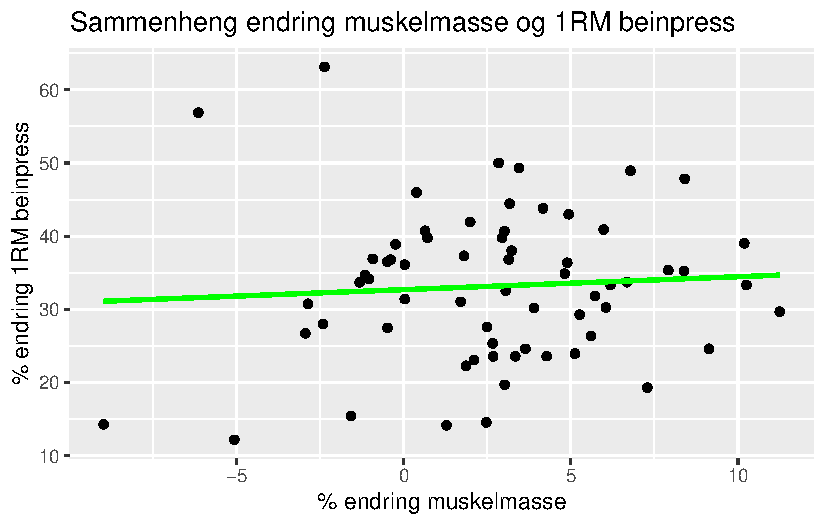
\includegraphics{05-repeated-measurements_files/figure-pdf/fig-figur1-1.pdf}

}

\caption{\label{fig-figur1}Figur som viser en lineær regresjonsmodell
med endring i muskelmasse som prediktor variabel for endring i 1RM
beinpress.}

\end{figure}%

\section{Diskusjon}\label{diskusjon-5}

I det beinet som trente tre sett, så man at det var mer hypertrofi og
større økning i styrke, målt i de to øvelsene, sammenlignet med de som
trente ett sett. Prosentvis endring i magermasse var høyere ved 3 sett,
henholdsvis 3.1 ± 4.4 \% mot ett sett, som økte 1.9 ± 3.5 \%. Man har
sett det samme i en metaanalyse, som så at to til tre sett og fire til
seks sett ga bedre resultat på effektstørrelse enn ett sett (ingen
forskjell mellom to til tre og fire til seks sett)\textsuperscript{22}.
Vi skal være litt forsiktige med å trekke konlusjoner basert på
metaanalyser, men mange andre studier sammenligner grupper med
forskjellige deltakere og ikke samme deltaker med ulikt treningsvolum på
to forskjellige bein\textsuperscript{23}. Dette gjør at man ikke får
tatt høyde for biologiske variasjoner hos de ulike individene, dermed
blir det vanskelig å sammenligne ulikt volum. Økningen i muskelmasse kan
i analysene fra denne rapporten ikke forklare økningen i 1 RM beinpress
når begge bein ble inkludert i korrelasjonsanalysen.

Til tross for at det ikke var noen sammenheng, så man også em større
økning i styrke, i beinpress ved tre sett kontra ett sett (den
prosentvise endringen på henholdsvis 34.4 ± 10.5 \& 31.9 ± 10). Man så
det samme på kneekstensjon, tre sett økte her 32.5 ± 9.1 \%, ett sett
derimot økte med 30.4 ± 8.8 \%.

Som konklusjon ut i fra de gjennomførte analysene fra rapporten, kan vi
si at responsen på styrke og hypertrofi følger et dose-volum forhold.
Dette vil si at tre sett er mer gunstig enn ett sett for ikke-røykende,
utrente kvinner og menn mellom 18 og 40 år.

\bookmarksetup{startatroot}

\chapter{Vitenskapsteori}\label{vitenskapsteori}

Induksjon er en prosess som blir brukt for å trekke konklusjoner basert
på observasjoner vi har gjort\textsuperscript{24}. Metoden, eller
prosessen blir gjerne brukt for å trekke generelle konklusjoner angående
hvordan verden er satt sammen og hvordan den fungerer. Konklusjonene
baserer seg på spesifikke observasjoner som har blitt gjort tidligere,
og observasjonene har gjerne blitt testet om igjen, og om igjen for å
sørge for at ting ikke har skjedd ved én tilfeldighet.

Det finnes både fullstendig og ufullstendig induksjon. Et eksempel på
fullstendig induksjon er ved valg, valgresultatet baserer seg på
induksjon. Alle stemmesedlene blir telt opp og vi kan konkludere med at
kandidaten som har fått flest stemmer, vinner valget. Ved fullstendig
induksjon kan vi være helt sikre på at konklusjonen vi har kommet frem
til er rett, siden vi har sett på alle stemmesedlene. Ved ufullstendig
induksjon baserer man seg på et begrenset antall observasjoner og
trekker en generell konklusjon deretter. Ved ufullstendig induksjon vil
det alltid være en fare for at konklusjonen er usann, siden man ikke
undersøker alle relevante tilfeller.

Hume mener på sin side at induksjon rett og slett ikke er så mye verdt.
I Humes´ øyne er det ingen logisk forklaring til at fremtiden vil
fortsette å være lik fortiden i all fremtid. Erfaringer vi har gjort oss
tidligere sier heller ikke noe om fremtiden, selv om det gir en god
pekepinn. Selv om to biler krasjer i et bestemt kryss i dag, betyr ikke
det at to biler vil krasje i det samme krysset i morgen. Hume
konkluderer med at induksjon kun er basert på vaner og/eller
forventninger og at det ikke er basert på rasjonell grunn.

En innvendig mot Humes premiss er at vi mennesker klarer å gjøre gode
resonnementer, gjenkjenne mønstre og tenke logisk. Med bakgrunn i dette
kan vi si at våre forventninger om fremtiden ikke kun er baser på
forventninger og vaner, men fra en dypere rasjonell forståelse av
verden. At ting har blitt som de har, er et resultat av den stadige
evolusjonen og utviklingen vi har hatt som menneskehet. Vi og verden har
utviklet oss for å stadig bedre vår overlevelsesevne. Og dermed vil vi
også fortsette å utvikle oss videre.

Hume ville i dette tilfellet antakelig svart med noe som at; selv om vi
i all tid så langt har utviklet oss som menneskehet, og verden stadig
har tatt fremskritt, betyr det ikke at vi vil fortsette med det i
morgen. Selv om all fornuft tyder på at morgendagen vil ligne på dagen i
går, siden dagen før der lignet på dagen i går, betyr det ikke at det
vil være sånn. Selv om vi mennesker har blitt gode på å kjenne igjen
mønstre, kan man fortsatt ikke forutse hvordan morgendagen blir. Det vet
vi kun i morgen.

Hovedessensen av prinsippet om falsifikasjon, eller falsifikasjonisme
handler om at vi i vitenskapen ikke bør prøve å finne argumenter for at
noe stemmer, men at vi heller bør prøve å falsifisere, altså bevise at
noe er usant. Karl Popper var opptatt av at teorier skulle kunne
motbevises ved hjelp av eksperimenter, eller observasjoner. Et eksempel
vi kan bruke fra idretten er teorien om at bruken av høydetrening kan
forbedre utholdenhetsprestasjonen. Hvis man har to forskjellige grupper,
en på høydetrening og en uten høydetrening. Og det ikke ses noen
forskjell i utholdenhetsprestasjon, kan hypotesen om høydetrening
falsifiseres. Hvis teorier kommer seg gjennom mange forsøk på
falsifikasjon, kan vi se på den som at den foreløpig er korrekt, men
aldri som endelig bekreftet. Popper gikk på sin side så langt, som å si
at søken etter bekreftelser på hypoteser er selve kjennetegnet på
pseudovitenskap.

Et problem med falsifikasjonisme, hentet fra idretten er effekten av
varmetrening på utholdenhetsprestasjon. Det har i dag blitt vanligere og
vanligere å drive med varmetrening, enten i oppvarmet rom eller ved bruk
av varmedrakt (for eksempel ullundertøy under regntøy). Det er mye
diskutert hva slags effekt dette kan ha på utholdenhetsprestasjonen,
også i konkurranser eller tester hvor det er normale forhold (hverken
oppvarmet rom eller varmedrakt i bruk). Det er en del andre variabler
som spiller inn her, spesielt individuelle forskjeller som gjøres blant
utøvere både underveis og i ettertid av en varmetreningsøkt. Eksempler
på dette er hydrering underveis og i etterkant, hvile og jern som
kosttilskudd. Dette gjør det vanskelig å teste denne hypotesen på en
falsifiserbar måte. En mulig løsning på dette problemet er å gjøre lange
kontrollerte studier der utøvere gjennomgår trening i varme forhold
(varmekammer/varmedrakt), med en stor nok kontrollgruppe som ikke gjør
noen form for varmetrening. I tillegg bør man i dette tilfellet sørge
for kontrollert oppfølging av både hydrering (sørge for at deltakerne
drikker lik mengde), hvile og andre faktorer som kan påvirke effekten av
varmetreningen. Dette er ulike tiltak som gjør at hypotesen blir mer
falsifiserbar.

Et annet eksempelproblem innenfor idrettsforskning og falsifikasjonisme
er som følger. Det settes opp et prosjekt som skal se på utvikling av
utholdenhet og styrke hos en rekke deltakere. Det gjøres baselinetester
før en treningsintervensjon på 12 uker. Etter de 12 ukene med trening er
gjennomført gjennomføres det nye tester for å se hvordan deltakerne nå
presterer. Halve gruppen har trent harde intervaller, og den andre
halvdelen har trent rolig trening. Gruppen som har gjennomført
intervalltrening har oppnådd mest fremgang, men problemet er at vi ikke
har tatt høyde for individuelle forskjeller blant deltakerne som er med.
En mulig løsning på dette problemet er at vi lar deltakerne få en 12
ukers washout-periode hvor det ikke blir gjennomført noe trening. Man
gjør nye baselinetester for å se om deltakerne nå har mistet
treningsadaptasjonene de opparbeidet seg i forkant. Vi gjennomfører nå
12 nye uker med trening, og deltakerne har nå byttet om, de som trente
intervalltrening under forrige intervensjon får nå rolig trening denne
gangen. På denne måten tar vi høyde for individuelle forskjeller,
ettersom vi nå har byttet om på deltakerne. Dette er en måte å gjøre
hypotesen mer falsifiserbar på.

Et tredje forsøk fra idrettsverden er placeboeffekt, det finnes mye
forskning gjort på kosttilskudd innenfor idretten. Hvis en utøver tror
man får et kosttilskudd som skal gi en forventet bedring i prestasjon
kan dette være nok til at man presterer bedre. Dette gjør det vanskelig
å falsifisere hypoteser. En mulig løsning på dette problemet er å gjøre
double blinded eller dobbeltblinda eksperimenter, så hverken forsker
eller forsøksperson vet om man får placebo eller om man får det faktiske
kosttilskuddet. Dette gjør hypotesen mer falsifiserbar, for hvis man i
dette tilfellet også finner effekt, kan man med ganske god sannsynlighet
si at det er på grunn av kosttilskuddets virkemiddel og ikke at utøveren
tror man har fått tilskuddet.

\bookmarksetup{startatroot}

\chapter{Lab-rapport}\label{lab-rapport}

\section{Introduksjon}\label{introduksjon-4}

Genekspresjonsanalyse med kvantitativ fluorescens-basert sanntids
polymerasekjedereaksjon (qPCR) er en avansert forskningsmetode som ofte
anvendes innen treningsfysiologi. Målet med qPCR er å studere genuttrykk
for et spesifikt målgen ved bruk av biologisk
materiale\textsuperscript{25}. qPCR er særlig nyttig for å måle
treningsinduserte endringer i genuttrykk i muskelfibertyper. Den største
forskjellen mellom qPCR og tradisjonell PCR er at qPCR gjør det mulig å
kvantifisere og måle mengden av DNA-sekvenser i
sanntid\textsuperscript{25}.

For å utføre qPCR kreves RNA, som ekstraheres fra biologisk materiale,
for eksempel muskelvev. RNA-et må gjennom flere trinn før det kan brukes
i analysen. Det første trinnet er å omdanne RNA til komplementært DNA
(cDNA) ved hjelp av en prosess som kalles revers
transkripsjon\textsuperscript{25}. Deretter kopieres cDNA eksponentielt,
slik at milliarder av kopier kan fremstilles\textsuperscript{25}.

\section{Metode}\label{metode-6}

Ved oppstart av forsøket fikk vi utdelt ferdigprodusert cDNA fra et
tidligere gjennomført styrketreningsprosjekt, levert av labansvarlig.
For å gjennomføre qPCR ble det brukt cDNA kombinert med en Master Mix,
som inneholdt følgende komponenter:

SYBR Green Mix: 50 µl Vann (H\(_2\)O): 20 µl Primer-mix (enten MHC1,
MHC2x eller MHC2a): 10 µl I tillegg ble det laget en kontroll-Master Mix
som besto av følgende:

b2m Primer-mix: 50 µl Vann (H\(_2\)O): 100 µl SYBR Green Mix: 250 µl
Fremstilling av fortynningsrekker

Under forsøket ble det også utarbeidet to ulike fortynningsrekker for å
standardisere og validere resultatene. Fortynningsrekkene var som
følger:

Fortynningsrekke 1: 1 (ufortynnet) 1/10 1/100 1/1000 Fortynningsrekke 2:
½ 1/20 1/200 For å lage fortynningsrekkene ble c-myc-primer fortynnet
med H\(_2\)O. I den ufortynnede prøven (1/1) ble det tilsatt 30 µl av
prøven og 0 µl H\(_2\)O, mens de resterende fortynningene ble fremstilt
ved proporsjonal tilsetning av vann og prøve.

Dette oppsettet sikret nøyaktighet og reproduserbarhet i analysen, og
tillot oss å undersøke genuttrykket under forskjellige
fortynningsforhold.

\begin{longtable}[]{@{}lrr@{}}
\caption{Fortynning Tabell}\tabularnewline
\toprule\noalign{}
Fortynning & Prøve & H2O \\
\midrule\noalign{}
\endfirsthead
\toprule\noalign{}
Fortynning & Prøve & H2O \\
\midrule\noalign{}
\endhead
\bottomrule\noalign{}
\endlastfoot
1 & 30 & 0 \\
1/10 & 2 & 18 \\
1/100 & 2 & 18 \\
1/1000 & 2 & 18 \\
½ & 10 & 10 \\
1/20 & 2 & 18 \\
1/200 & 2 & 18 \\
\end{longtable}

Flytter 2 µl fra rør 1 til 2a, og 10µl fra 1 til 2b, vortex rør 2a+2b.

Flytter 2µl fra 2a til 3a og 2µl fra 2b til 3b, vortex rør 3a+3b.

Flytter 2µl fra 3a til 4a og 2µ fra 3b til 4b, vortex rør 4a + 4b.

\begin{longtable}[]{@{}
  >{\raggedright\arraybackslash}p{(\columnwidth - 18\tabcolsep) * \real{0.0366}}
  >{\raggedright\arraybackslash}p{(\columnwidth - 18\tabcolsep) * \real{0.1341}}
  >{\raggedright\arraybackslash}p{(\columnwidth - 18\tabcolsep) * \real{0.1585}}
  >{\raggedright\arraybackslash}p{(\columnwidth - 18\tabcolsep) * \real{0.0854}}
  >{\raggedright\arraybackslash}p{(\columnwidth - 18\tabcolsep) * \real{0.0976}}
  >{\raggedright\arraybackslash}p{(\columnwidth - 18\tabcolsep) * \real{0.0976}}
  >{\raggedright\arraybackslash}p{(\columnwidth - 18\tabcolsep) * \real{0.0976}}
  >{\raggedright\arraybackslash}p{(\columnwidth - 18\tabcolsep) * \real{0.0976}}
  >{\raggedright\arraybackslash}p{(\columnwidth - 18\tabcolsep) * \real{0.0976}}
  >{\raggedright\arraybackslash}p{(\columnwidth - 18\tabcolsep) * \real{0.0976}}@{}}
\caption{Tabell: Oversikt over prøver}\tabularnewline
\toprule\noalign{}
\begin{minipage}[b]{\linewidth}\raggedright
\end{minipage} & \begin{minipage}[b]{\linewidth}\raggedright
Pre\_week\_0
\end{minipage} & \begin{minipage}[b]{\linewidth}\raggedright
Post\_week\_12
\end{minipage} & \begin{minipage}[b]{\linewidth}\raggedright
cmyc\_1
\end{minipage} & \begin{minipage}[b]{\linewidth}\raggedright
cmyc\_2a
\end{minipage} & \begin{minipage}[b]{\linewidth}\raggedright
cmyc\_3a
\end{minipage} & \begin{minipage}[b]{\linewidth}\raggedright
cmyc\_4a
\end{minipage} & \begin{minipage}[b]{\linewidth}\raggedright
cmyc\_2b
\end{minipage} & \begin{minipage}[b]{\linewidth}\raggedright
cmyc\_3b
\end{minipage} & \begin{minipage}[b]{\linewidth}\raggedright
cmyc\_4b
\end{minipage} \\
\midrule\noalign{}
\endfirsthead
\toprule\noalign{}
\begin{minipage}[b]{\linewidth}\raggedright
\end{minipage} & \begin{minipage}[b]{\linewidth}\raggedright
Pre\_week\_0
\end{minipage} & \begin{minipage}[b]{\linewidth}\raggedright
Post\_week\_12
\end{minipage} & \begin{minipage}[b]{\linewidth}\raggedright
cmyc\_1
\end{minipage} & \begin{minipage}[b]{\linewidth}\raggedright
cmyc\_2a
\end{minipage} & \begin{minipage}[b]{\linewidth}\raggedright
cmyc\_3a
\end{minipage} & \begin{minipage}[b]{\linewidth}\raggedright
cmyc\_4a
\end{minipage} & \begin{minipage}[b]{\linewidth}\raggedright
cmyc\_2b
\end{minipage} & \begin{minipage}[b]{\linewidth}\raggedright
cmyc\_3b
\end{minipage} & \begin{minipage}[b]{\linewidth}\raggedright
cmyc\_4b
\end{minipage} \\
\midrule\noalign{}
\endhead
\bottomrule\noalign{}
\endlastfoot
A & myhe 1 & myhe 1 & NA & NA & NA & NA & NA & NA & NA \\
B & myhe 1 & myhe 1 & NA & NA & NA & NA & NA & NA & NA \\
C & myhe 1 & myhe 1 & NA & NA & NA & NA & NA & NA & NA \\
D & myhe 2a & myhe 2a & NA & NA & NA & NA & NA & NA & NA \\
E & myhe 2a & myhe 2a & NA & NA & NA & NA & NA & NA & NA \\
F & myhe 2a & myhe 2a & NA & NA & NA & NA & NA & NA & NA \\
G & myhe 2x & myhe 2x & NA & NA & NA & NA & NA & NA & NA \\
H & myhe 2x & myhe 2x & NA & NA & NA & NA & NA & NA & NA \\
I & myhe 2x & myhe 2x & NA & NA & NA & NA & NA & NA & NA \\
J & b2m & b2m & NA & NA & NA & NA & NA & NA & NA \\
K & b2m & b2m & NA & NA & NA & NA & NA & NA & NA \\
L & b2m & b2m & NA & NA & NA & NA & NA & NA & NA \\
\end{longtable}

Prøvene ble pipettert over i brønner i henhold til et forhåndsdefinert
pipetteringskart. Hver brønn ble fylt med 8 µl primer-spesifikk prøve og
2 µl cDNA-løsning eller kontrolløsning (A-L, 1 og 2). Fortynningsrekkene
ble pipettert inn i brønnene 5-11 (A-C). Alle prøvene ble satt opp i et
treplat-format, noe som sikret nøyaktighet og reproduserbarhet i
analysen.

qPCR-analysen ble gjennomført ved hjelp av Applied Biosystems 7500 Fast
Real-Time PCR System (Life Technologies AS) og programvaren Quant Studio
5. Prosessen besto av tre hovedtrinn. Først ble prøvene kjørt i en «Hold
stage» der temperaturen økte med 1,99 °C/s opp til 50 °C, hvor den ble
holdt konstant i 2 minutter. Deretter økte temperaturen videre med 1,99
°C/s opp til 95 °C, hvor den ble holdt i ytterligere 2 minutter.

Selve PCR-prosessen, kalt «PCR stage», besto av 40 sykluser. Hver syklus
innebar at temperaturen først ble holdt på 95 °C i 1 sekund før den
senket seg med 1,77 °C/s til 60 °C. Denne temperaturen ble deretter
holdt konstant i 30 sekunder. Etter hver syklus ble det tatt et bilde av
fluorescensen for å overvåke reaksjonen i sanntid.

Til slutt ble prøvene kjørt gjennom en «Melt stage». Her økte
temperaturen med 1,99 °C/s opp til 95 °C, hvor den ble holdt i 15
sekunder. Deretter ble temperaturen gradvis senket med 1,77 °C/s til 60
°C, hvor den ble holdt konstant i 1 minutt. Til slutt økte temperaturen
med 0,15 °C/s opp til 95 °C igjen, hvor den ble holdt i 15 sekunder.
Etter dette var PCR-prosessen ferdig, og CT-verdiene ble hentet ut for
videre analyse.

\subsection{Databehandling}\label{databehandling}

De innsamlede CT-verdiene ble analysert og behandlet ved hjelp av
Microsoft Excel. Dette inkluderte utregninger og datavisualisering for å
tolke genuttrykk og endringer i fluorescens. Hele prosessen sikret
presise resultater og pålitelige konklusjoner.

\begin{longtable}[t]{>{}l>{}l>{}r>{}r>{}r>{}r}
\caption{Ct-verdier for de ulike prøvene}\\
\toprule
\multicolumn{1}{c}{ } & \multicolumn{5}{c}{Ct Data} \\
\cmidrule(l{3pt}r{3pt}){2-6}
Sample Name & Target Name & Ct1 & Ct2 & Ct3 & Average Ct\\
\midrule
Control sample W0 & b2m & 23.427 & 24.072 & 23.318 & 23.60567\\
W0 & MHC I & 18.299 & 19.223 & 19.764 & 19.09533\\
W12 & MHC I & 18.431 & 19.080 & 18.348 & 18.61967\\
W0 & MHC 2a & 22.419 & 17.707 & 18.314 & 19.48000\\
W12 & MHC 2a & 18.393 & 18.731 & 35.236 & 24.12000\\
\addlinespace
W0 & MHC 2x & 25.708 & 25.036 & 23.771 & 24.83833\\
W12 & MHC 2x & 25.120 & 23.575 & 23.052 & 23.91567\\
\bottomrule
\end{longtable}

Tallene viser til antall sykluser før syklisk terskel (CT) er nådd. CT
verdiene verdier for å nå syklisk terskel har endret seg fra uke 0 til
uke 12. For MHC1 har det endret seg fra et gjennomsnitt på 19,09 -18,62
sykluser. For MHC2a har det endret seg fra 19,48 -24,12 og for MHC 2x
fra 24,83-23,91. Et lavere antall sykluser et større genutrykk.

\begin{longtable*}[t]{>{}lrrr}
\toprule
\multicolumn{1}{c}{ } & \multicolumn{3}{c}{Prosentvis fordeling av genuttrykk} \\
\cmidrule(l{3pt}r{3pt}){2-4}
Uke & MHC1 & MHC2a & MHC2x\\
\midrule
\textbf{Uke 0} & 56 & 43 & 1\\
\textbf{Uke 12} & 95 & 2 & 2\\
\bottomrule
\end{longtable*}

Vi ser at mengden genuttrykk for muskelfibertype 2a (MHC-2a) har sunket
fra 43\% til 2\% etter 12 uker, det har også vært en reduksjon for
muskelfibertype 2x (MHC-2x) fra 2\% til 1\%. Muskelfibertype 1 (MHC1)
har derimot økt fra 56\% til 95\%.

\begin{longtable}[t]{>{}rr}
\caption{Primer Efficiency Results}\\
\toprule
Slope & Primer Efficiency\\
\midrule
\textbf{-2.477405} & 153.31\\
\bottomrule
\end{longtable}

\section{Diskusjon}\label{diskusjon-6}

Målet med dette forsøket var å undersøke endringer i myoisintungkjedene.
Etter en styrketreningsintevesjon på utrent forsøksperson på 12 uker,
ved hjelp av fluoricens- basert sanntids kvantitativ polymerase
kjedereaksjon (qPCR).

Det har i dette forsøket blitt undersøkt hvor mange sykluser CT-verdiene
til den ulike myoisintungkjedene trenger for å nå sin terskelverdi. Der
færre sykluser og lavere CT verdier indikerer et størrre genutrykk. I
våre resulatater har vi sett en endring for alle myosintunkjedene når
det gjelder antall sykluser myoisnkjedene har trengt for å nå sin
CT-verdi og den prosentvise endringen for tungkjedene indikerer at vi
har fått en stor endring fra 56\%- 95\% for MHCI, for MHC2a har det
blitt redusert fra 43\% til 2\%, det samme gjelder for MHC2x som har
fått en reduksjon fra 2\%-1\%.

I en tidligere studie av Ellefsen et al.~(2014), hvor en
styrketreningsintervensjon ble gjennomført på utrente individer over 12
uker, ble det observert en økning i MHC2A, en reduksjon i MHC2X, samt
stabilitet i MHC1\textsuperscript{26}. I kontrast til dette viser våre
resultater motstridende funn, med både reduksjon i MHC2A og MHC2X, samt
en betydelig økning i MHC1. Andre studier, som\textsuperscript{27}
Terzis et al. (2008) og\textsuperscript{28} også vist at utrente
personer med overvekt av MHC2X opplever en reduksjon i MHC2X og en
økning i MHC2A ved trening, med minimal endring i MHC1. Det er kjent at
genuttrykk ikke kan endres fra MHC1 til MHC2A eller MHC2X, noe som gjør
det vanskelig å forklare de resultatene vi har fått fra analysen av
myosintungkjeder. Dette reiser spørsmål om hva som kan ha skjedd under
vår analyse og om det er spesifikke faktorer ved vårt eksperiment som
kan ha bidratt til disse avvikene fra tidligere forskning.

Det som en kan reise en usikkerhet om er om både pippetringferdigheter
og primerkvaliteten har vært god nok enten at primer har gått ut på dato
eller bruk av feil primer. Primer efficency skulle ligge mellom
90-110\%. I vårt tilfelle fikk vi en efficency på 153\% noe som kan tyde
på at det kan være menneskelige feil som har påvirket resulatet. Det er
også vanskelig å skulle trekke slutninger basert på en prøve. Samt at vi
har ingen forkunnskap om hvilket treningsstimuli forsøkspersonen vi har
fått har vært utsatt for, annet enn den informasjonen vi har fått fra
labansvarlig.

\subsection{Konklusjon}\label{konklusjon-1}

Basert på funn vi har fått i forsøket kan vi ikke si noe om endringene i
myiosntungkjedene for denne forsøkspersonen. Da resultatene vi har fått
ikke er mulig basert på det vi kjenner til av tidligere forskning.

\bookmarksetup{startatroot}

\chapter*{Referanser}\label{referanser}
\addcontentsline{toc}{chapter}{Referanser}

\phantomsection\label{refs}
\begin{CSLReferences}{1}{0}
\bibitem[\citeproctext]{ref-RN130}
1. Hopkins, W. G. (2000). Measures of reliability in sports medicine and
science {[}Journal Article{]}. \emph{Sports Med}, \emph{30}(1), 1--15.
\url{http://www.ncbi.nlm.nih.gov/pubmed/10907753}

\bibitem[\citeproctext]{ref-Spiegelhalter}
2. Spiegelhalter, D. (2020). Introducing the art of statistics: How to
learn from data. \emph{Numeracy}, \emph{13}(1).

\bibitem[\citeproctext]{ref-Bassett}
3. Bassett, D. R., Jr, \& Howley, E. T. (2000). Limiting factors for
maximum oxygen uptake and determinants of endurance performance.
\emph{Med. Sci. Sports Exerc.}, \emph{32}(1), 70--84.

\bibitem[\citeproctext]{ref-Joyner}
4. Joyner, M. J., \& Coyle, E. F. (2008). Endurance exercise
performance: The physiology of champions. \emph{J. Physiol.},
\emph{586}(1), 35--44.

\bibitem[\citeproctext]{ref-RN2511}
5. Tanner, R. K., \& Gore, C. J. (2012). \emph{Physiological tests for
elite athletes 2nd edition} {[}Book{]}. Human Kinetics.
\url{https://books.google.no/books?id=0OPIiMks58MC}

\bibitem[\citeproctext]{ref-Halperin}
6. Halperin, I., Pyne, D. B., \& Martin, D. T. (2015). Threats to
internal validity in exercise science: A review of overlooked
confounding variables. \emph{Int. J. Sports Physiol. Perform.},
\emph{10}(7), 823--829.

\bibitem[\citeproctext]{ref-Pisica2022}
7. Pisică, D., Dammers, R., Boersma, E., \& Volovici, V. (2022). Tenets
of good practice in regression analysis. A brief tutorial. \emph{World
Neurosurg.}, \emph{161}, 230--239.e6.

\bibitem[\citeproctext]{ref-machado2012}
8. Machado, F. A., Nakamura, F. Y., \& Moraes, S. M. F. D. (2012).
Influence of regression model and incremental test protocol on the
relationship between lactate threshold using the maximal-deviation
method and performance in female runners. \emph{Journal of Sports
Sciences}, \emph{30}(12), 1267--1274.
\url{https://doi.org/10.1080/02640414.2012.702424}

\bibitem[\citeproctext]{ref-Ronnestad2014-bu}
9. Rønnestad, B. R., Hansen, J., \& Ellefsen, S. (2014). Block
periodization of high-intensity aerobic intervals provides superior
training effects in trained cyclists. \emph{Scand. J. Med. Sci. Sports},
\emph{24}(1), 34--42.

\bibitem[\citeproctext]{ref-Ronnestad2014-xg}
10. Rønnestad, B. R., Ellefsen, S., Nygaard, H., Zacharoff, E. E.,
Vikmoen, O., Hansen, J., \& Hallén, J. (2014). Effects of 12 weeks of
block periodization on performance and performance indices in
well-trained cyclists. \emph{Scand. J. Med. Sci. Sports}, \emph{24}(2),
327--335.

\bibitem[\citeproctext]{ref-Breil2010-mr}
11. Breil, F. A., Weber, S. N., Koller, S., Hoppeler, H., \& Vogt, M.
(2010). Block training periodization in alpine skiing: Effects of 11-day
{HIT} on {VO2max} and performance. \emph{Eur. J. Appl. Physiol.},
\emph{109}(6), 1077--1086.

\bibitem[\citeproctext]{ref-Ronnestad2016-nq}
12. Rønnestad, B. R., Hansen, J., Thyli, V., Bakken, T. A., \& Sandbakk,
Ø. (2016). 5-week block periodization increases aerobic power in elite
cross-country skiers. \emph{Scand. J. Med. Sci. Sports}, \emph{26}(2),
140--146.

\bibitem[\citeproctext]{ref-Solli2019-ej}
13. Solli, G. S., Tønnessen, E., \& Sandbakk, Ø. (2019). Block vs.
Traditional periodization of {HIT}: Two different paths to success for
the world's best cross-country skier. \emph{Front. Physiol.}, \emph{10},
375.

\bibitem[\citeproctext]{ref-carpinelli1998}
14. Carpinelli, R. N., \& Otto, R. M. (1998). Strength Training: Single
Versus Multiple Sets. \emph{Sports Medicine}, \emph{26}(2), 73--84.
\url{https://doi.org/10.2165/00007256-199826020-00002}

\bibitem[\citeproctext]{ref-sooneste2013}
15. Sooneste, H., Tanimoto, M., Kakigi, R., Saga, N., \& Katamoto, S.
(2013). Effects of Training Volume on Strength and Hypertrophy in Young
Men. \emph{Journal of Strength and Conditioning Research}, \emph{27}(1),
8--13. \url{https://doi.org/10.1519/JSC.0b013e3182679215}

\bibitem[\citeproctext]{ref-radaelli2015}
16. Radaelli, R., Fleck, S. J., Leite, T., Leite, R. D., Pinto, R. S.,
Fernandes, L., \& Simão, R. (2015). Dose-Response of 1, 3, and 5 Sets of
Resistance Exercise on Strength, Local Muscular Endurance, and
Hypertrophy. \emph{Journal of Strength and Conditioning Research},
\emph{29}(5), 1349--1358.
\url{https://doi.org/10.1519/JSC.0000000000000758}

\bibitem[\citeproctext]{ref-cannon2010}
17. Cannon, J., \& Marino, F. E. (2010). Early-phase neuromuscular
adaptations to high- and low-volume resistance training in untrained
young and older women. \emph{Journal of Sports Sciences}, \emph{28}(14),
1505--1514. \url{https://doi.org/10.1080/02640414.2010.517544}

\bibitem[\citeproctext]{ref-mitchell2012}
18. Mitchell, C. J., Churchward-Venne, T. A., West, D. W. D., Burd, N.
A., Breen, L., Baker, S. K., \& Phillips, S. M. (2012). Resistance
exercise load does not determine training-mediated hypertrophic gains in
young men. \emph{Journal of Applied Physiology}, \emph{113}(1), 71--77.
\url{https://doi.org/10.1152/japplphysiol.00307.2012}

\bibitem[\citeproctext]{ref-marx2001}
19. Marx, J. O., Ratamess, N. A., Nindl, B. C., Gotshalk, L. A., Volek,
J. S., Dohi, K., Bush, J. A., G??Mez, A. L., Mazzetti, S. A., Fleck, S.
J., H??Kkinen, K., Newton, R. U., \& Kraemer, W. J. (2001). Low-volume
circuit versus high-volume periodized resistance training in women:
\emph{Medicine and Science in Sports and Exercise}, 635--643.
\url{https://doi.org/10.1097/00005768-200104000-00019}

\bibitem[\citeproctext]{ref-messier1985}
20. Messier, S. P., \& Dill, M. E. (1985). Alterations in Strength and
Maximal Oxygen Uptake Consequent to Nautilus Circuit Weight Training.
\emph{Research Quarterly for Exercise and Sport}, \emph{56}(4),
345--351. \url{https://doi.org/10.1080/02701367.1985.10605339}

\bibitem[\citeproctext]{ref-rstudio}
21. Posit team. (2023). \emph{RStudio: Integrated development
environment for r}. Posit Software, PBC. \url{http://www.posit.co/}

\bibitem[\citeproctext]{ref-krieger2009}
22. Krieger, J. W. (2009). Single Versus Multiple Sets of Resistance
Exercise: A Meta-Regression. \emph{Journal of Strength and Conditioning
Research}, \emph{23}(6), 1890--1901.
\url{https://doi.org/10.1519/JSC.0b013e3181b370be}

\bibitem[\citeproctext]{ref-starkey1996}
23. Starkey, D. B., Pollock, M. L., Ishida, Y., Welsch, M. A., Brechue,
W. F., Graves, J. E., \& Feigenbaum, M. S. (1996). Effect of resistance
training volume on strength and muscle thickness: \emph{Medicine \&
Science in Sports \& Exercise}, \emph{28}(10), 1311--1320.
\url{https://doi.org/10.1097/00005768-199610000-00016}

\bibitem[\citeproctext]{ref-Thuren2022-vp}
24. Thurén, T. (2022). \emph{Vitenskapsteori for nybegynnere}.

\bibitem[\citeproctext]{ref-kuang2018}
25. Kuang, J., Yan, X., Genders, A. J., Granata, C., \& Bishop, D. J.
(2018). An overview of technical considerations when using quantitative
real-time PCR analysis of gene expression in human exercise research.
\emph{PLOS ONE}, \emph{13}(5), e0196438.
\url{https://doi.org/10.1371/journal.pone.0196438}

\bibitem[\citeproctext]{ref-ellefsen2014}
26. Ellefsen, S., Vikmoen, O., Zacharoff, E., Rauk, I., Slettaløkken,
G., Hammarström, D., Strand, T. A., Whist, J. E., Hanestadhaugen, M.,
Vegge, G., Fagernes, C. E., Nygaard, H., Hollan, I., \& Rønnestad, B. R.
(2014). Reliable determination of training-induced alterations in muscle
fiber composition in human skeletal muscle using quantitative polymerase
chain reaction. \emph{Scandinavian Journal of Medicine \& Science in
Sports}, \emph{24}(5). \url{https://doi.org/10.1111/sms.12185}

\bibitem[\citeproctext]{ref-terzis2008}
27. Terzis, G., Georgiadis, G., Stratakos, G., Vogiatzis, I., Kavouras,
S., Manta, P., Mascher, H., \& Blomstrand, E. (2008). Resistance
exercise-induced increase in muscle mass correlates with p70S6 kinase
phosphorylation in human subjects. \emph{European Journal of Applied
Physiology}, \emph{102}(2), 145--152.
\url{https://doi.org/10.1007/s00421-007-0564-y}

\bibitem[\citeproctext]{ref-andersen2000}
28. Andersen, J. L., \& Aagaard, P. (2000). Myosin heavy chain IIX
overshoot in human skeletal muscle. \emph{Muscle \& Nerve},
\emph{23}(7), 1095--1104.
\url{https://doi.org/10.1002/1097-4598(200007)23:7\%3C1095::AID-MUS13\%3E3.0.CO;2-O}

\end{CSLReferences}




\end{document}
